% Options for packages loaded elsewhere
\PassOptionsToPackage{unicode}{hyperref}
\PassOptionsToPackage{hyphens}{url}
%
\documentclass[
  10,
  spanish,
  openany]{book}
\title{Sistema Complementario Saber UCV (SCSU): recuperación de datos desde PDF, clasificación y construcción de un repositorio en línea}
\usepackage{etoolbox}
\makeatletter
\providecommand{\subtitle}[1]{% add subtitle to \maketitle
  \apptocmd{\@title}{\par {\large #1 \par}}{}{}
}
\makeatother
\subtitle{Caso de Estudio Repositorio www.saber.ucv.ve}
\author{José Miguel Avendaño Infante}
\date{2022-02-03}

\usepackage{amsmath,amssymb}
\usepackage{lmodern}
\usepackage{iftex}
\ifPDFTeX
  \usepackage[T1]{fontenc}
  \usepackage[utf8]{inputenc}
  \usepackage{textcomp} % provide euro and other symbols
\else % if luatex or xetex
  \usepackage{unicode-math}
  \defaultfontfeatures{Scale=MatchLowercase}
  \defaultfontfeatures[\rmfamily]{Ligatures=TeX,Scale=1}
  \setmainfont[]{Times New Roman}
\fi
% Use upquote if available, for straight quotes in verbatim environments
\IfFileExists{upquote.sty}{\usepackage{upquote}}{}
\IfFileExists{microtype.sty}{% use microtype if available
  \usepackage[]{microtype}
  \UseMicrotypeSet[protrusion]{basicmath} % disable protrusion for tt fonts
}{}
\makeatletter
\@ifundefined{KOMAClassName}{% if non-KOMA class
  \IfFileExists{parskip.sty}{%
    \usepackage{parskip}
  }{% else
    \setlength{\parindent}{0pt}
    \setlength{\parskip}{6pt plus 2pt minus 1pt}}
}{% if KOMA class
  \KOMAoptions{parskip=half}}
\makeatother
\usepackage{xcolor}
\IfFileExists{xurl.sty}{\usepackage{xurl}}{} % add URL line breaks if available
\IfFileExists{bookmark.sty}{\usepackage{bookmark}}{\usepackage{hyperref}}
\hypersetup{
  pdftitle={Sistema Complementario Saber UCV (SCSU): recuperación de datos desde PDF, clasificación y construcción de un repositorio en línea},
  pdfauthor={José Miguel Avendaño Infante},
  pdflang={es-ES},
  hidelinks,
  pdfcreator={LaTeX via pandoc}}
\urlstyle{same} % disable monospaced font for URLs
\usepackage[left=2.54cm, right=2.54cm, top=2.54cm, bottom=2.54cm]{geometry}
\usepackage{longtable,booktabs,array}
\usepackage{calc} % for calculating minipage widths
% Correct order of tables after \paragraph or \subparagraph
\usepackage{etoolbox}
\makeatletter
\patchcmd\longtable{\par}{\if@noskipsec\mbox{}\fi\par}{}{}
\makeatother
% Allow footnotes in longtable head/foot
\IfFileExists{footnotehyper.sty}{\usepackage{footnotehyper}}{\usepackage{footnote}}
\makesavenoteenv{longtable}
\usepackage{graphicx}
\makeatletter
\def\maxwidth{\ifdim\Gin@nat@width>\linewidth\linewidth\else\Gin@nat@width\fi}
\def\maxheight{\ifdim\Gin@nat@height>\textheight\textheight\else\Gin@nat@height\fi}
\makeatother
% Scale images if necessary, so that they will not overflow the page
% margins by default, and it is still possible to overwrite the defaults
% using explicit options in \includegraphics[width, height, ...]{}
\setkeys{Gin}{width=\maxwidth,height=\maxheight,keepaspectratio}
% Set default figure placement to htbp
\makeatletter
\def\fps@figure{htbp}
\makeatother
\setlength{\emergencystretch}{3em} % prevent overfull lines
\providecommand{\tightlist}{%
  \setlength{\itemsep}{0pt}\setlength{\parskip}{0pt}}
\setcounter{secnumdepth}{5}
\usepackage{booktabs}
\usepackage{longtable}
\usepackage[none]{hyphenat}
\raggedbottom
\usepackage{blindtext}
\usepackage[utf8]{inputenc}

\usepackage{scrlayer-scrpage}
\usepackage{lipsum}% just to generate text for the example

\pagestyle{scrheadings}
\clearpairofpagestyles
\ohead{\rightmark}
\cfoot[\pagemark]{\pagemark}



\let\oldmaketitle\maketitle
\AtBeginDocument{\let\maketitle\relax}
\usepackage{booktabs}
\usepackage{longtable}
\usepackage{array}
\usepackage{multirow}
\usepackage{wrapfig}
\usepackage{float}
\usepackage{colortbl}
\usepackage{pdflscape}
\usepackage{tabu}
\usepackage{threeparttable}
\usepackage{threeparttablex}
\usepackage[normalem]{ulem}
\usepackage{makecell}
\usepackage{xcolor}
\usepackage{fontspec}
\usepackage{multicol}
\usepackage{hhline}
\usepackage{hyperref}
\ifXeTeX
  % Load polyglossia as late as possible: uses bidi with RTL langages (e.g. Hebrew, Arabic)
  \usepackage{polyglossia}
  \setmainlanguage[]{spanish}
\else
  \usepackage[main=spanish]{babel}
% get rid of language-specific shorthands (see #6817):
\let\LanguageShortHands\languageshorthands
\def\languageshorthands#1{}
\fi
\ifLuaTeX
  \usepackage{selnolig}  % disable illegal ligatures
\fi
\usepackage[]{natbib}
\bibliographystyle{apalike}

\begin{document}
\maketitle

%\vspace{-2.0cm}
\pagenumbering{roman}

\begin{center}
	UNIVERSIDAD CENTRAL DE VENEZUELA\\
	FACULTAD DE CIENCIAS\\
	POSTGRADO EN CIENCIAS DE LA COMPUTACI\'ON\\

	\begin{figure}
						\centering
						  
\includegraphics[height=.7\textwidth]{images/UCV.png}
  \end{figure}
  \vspace{1.5cm}
  \large{\textbf{ANTEPROYECTO:\\ Solución Sistema Complementario Saber UCV (SSCSU): extracción de datos desde PDF, clasificación y construcción de un sistema de recuperación de información en línea}}

  \vspace{3cm}
  Anteproyecto presentado  \\
  por el Econ. José Miguel Avendaño Infante\\
  Tutor: Dr. Andrés Sanoja\\
  \vspace{1.5cm}
  Caracas, Octubre de 2021
\end{center}




%\newpage


\setlength{\abovedisplayskip}{-5pt}
\setlength{\abovedisplayshortskip}{-5pt}
\thispagestyle{empty}

\thispagestyle{empty}

\newpage
\thispagestyle{empty}
\large{\textbf{Resumen:}}

Se presenta la propuesta de un sistema denominado **Solución Sistema Complementario Saber UCV (SSCSU)** para hacer procesos de Recuperación de Información sobre los Resúmenes, tanto de las Tesis como de los Trabajos Especiales de Grado (TEG), que se encuentran alojados en el repositorio institucional Saber UCV (www.saber.ucv.ve).

Se aplican técnicas de Procesamiento de Lenguaje Natural (NLP), de Minería de Texto y de indexación en base de datos sobre los textos.

Esta propuesta se basa en que mediante la búsqueda de palabras o frases, aplicando filtros y determinando la granularidad, se genere un (*query*) con el que se puedan recuperar los trabajos en que se encuentran contenidas tales palabras y  a partir de ahí enriquecer la experiencia del usuario con la presentación de la información recuperada en tablas interactivas, visualizaciones con gráficos y grafos de coocurrencia de palabras.

La aplicación se diseña como un sistema distribuido bajo la arquitectura cliente-servidor y se soporta en el uso de contenedores, donde en cada uno se ejecuta un proceso para el funcionamiento de la SSCSU, siendo los principales el de la base de datos, el servidor de la aplicación y otro con los distintos procesamientos que son efectuados sobre los textos.

También se propone una rutina que permite clasificar las Tesis y los TEG por el área académica donde cursó estudios el autor del correspondiente trabajo y así se solventa la carencia que actualmente presenta Saber UCV, donde no están disponibles estas clasificaciones.

\thispagestyle{empty}

\maketitle



{
\setcounter{tocdepth}{3}
\tableofcontents
}
\listoffigures
\listoftables
\clearpage
\pagenumbering{arabic}

\hypertarget{section}{%
\chapter*{\_\_\_}\label{section}}
\addcontentsline{toc}{chapter}{\_\_\_}

\begin{quote}
Every important aspect of programming arises somewhere in the context of sorting or searching.

--- Donald Knuth, The Art of Computer Programming, Volume 3
\end{quote}

\hypertarget{introduccion}{%
\chapter{Introducción}\label{introduccion}}

En este Capítulo se presenta la Propuesta \ref{propuesta} denominada \textbf{Solución Sistema Complementario Saber UCV (SSCSU)}. Posteriormente se introducen los \textbf{Sistemas de Recuperación de Información} \ref{intro} y el repositorio institucional de documentos electrónicos \textbf{Saber UCV} \ref{saber}. Seguidamente se delimitan los documentos de Saber UCV con los que se trabajará en \ref{corpus}. En \ref{requerimiento} se expone el requerimiento inicial efectuado dentro del Postgrado de Ciencias de la Computación que motivó la realización de este desarrollo y se muestran los impedimentos y limitaciones en \ref{problema}, dadas las características de \textbf{Saber UCV}, que era necesario superar para cumplir con el requerimiento y poder desarrollar esta Propuesta. Igualmente se hace un repaso a investigaciones llevadas a cabo \ref{antecedentes} en la Universidad Central de Venezuela, que parcialmente han abordado problemas y soluciones similares a la que acá se presenta. Finalmente se detalla la estructura \ref{estructura} por capítulos de este Anteproyecto.

\hypertarget{propuesta}{%
\section{Propuesta:}\label{propuesta}}

En este trabajo se formula la propuesta de una Solución que permite realizar procesos de \textbf{Recuperación de Información} \ref{infret} sobre los Resúmenes, tanto de las Tesis como de los Trabajos Especiales de Grado, que están alojados en el repositorio institucional de documentos digitales ``Saber U.C.V.'' de la Universidad Central de Venezuela.

La propuesta se basa en el desarrollo e implementación de un sistema distribuido con una arquitectura cliente-servidor, disponiendo de una aplicación web donde el cliente accede usando el navegador web. Al usuario se le permitirá hacer la formulación de una consulta para filtrar, dentro de un conjunto de textos, aquellos que cumplen las condiciones definidas.

La consulta, a la cual denominaremos el \textbf{query}, estará definida por: una frase, la selección de diversos criterios para el filtrado de los datos y la selección de la granularidad \footnote{En la inteligencia de negocios el término granularidad hace referencia al nivel de detalle, o sumarización de las unidades de datos que reposan en el \emph{data warehouse} , a más detalle, menos es la granularidad y a menor detalle implica una mayor granularidad \citep{inmon2002}. En el campo de la recuperación de información este término se contextualiza en el nivel de detalle al que llegará la recuperación dentro de un texto, pudiendo ser por ejemplo dentro de un documento la búsqueda de una ocurrencia, dentro de un capítulo, de una sección, de un párrafo o de una oración. Una de las formas en que serán representados los resultados obtenidos, mediante la coocurrencia de palabras, mostrará distintas granularidades tanto en parrafos como en el texto completo del resumen de la tesis. Igualmente se asocia la granularidad a la restricción que se podrá seleccionar para hacer la búsqueda, delimitando si se quiere buscar dentro de todas las facultades, en alguna de ellas, o sólo documentos dentro producidos dentro de una escuela y/o postgrado.}, \emph{eg.} un intervalo de fechas, la selección de la(s) facultad(es) y/o escuela(s)-postgrado(s) donde se generó la investigación. Al ejecutar la consulta serán recuperados del Sistema los textos que cumplen con las restricciones establecidas. Los resultados se mostrarán con distintos gráficos, tablas interactivas, grafos de coocurrencia de palabras \ref{coocurrencia} y recomendaciones de documentos, basados en las similitudes que pueda presentar un documento con los otros \ref{similitud}. La propuesta descrita recibirá el nombre de \textbf{Solución Sistema Complementario Saber UCV (SSCSU)}.

La SSCSU será desarrollada basándose en los principios que definen a los Sistemas de Recuperación de Información \ref{SRI} y se conformará un conjunto delimitado de documentos con los resumenes, lo cual en la literatura especializada se denomina el \emph{Corpus} \ref{corpus}. Sobre este conjunto serán aplicadas técnicas de Minería de Texto \ref{textmin} y de Procesamiento de Lenguaje Natural \ref{nlproc}, para detectar relaciones entre los elementos y extraer conocimiento de los mismos \citep{miningt2012c}.

La implementación del Sistema se hará mediante el uso de contenedores encargados de sustentar los procesos medulares y complementarios. Entre los procesos medulares se encuentran los de gestión de la base de datos, el servidor de la aplicación y el de procesamientos de los textos \footnote{La creación de los contenedores y la integración de estos se hará mediante el uso de \emph{Docker} y \emph{Docker Compose} respectivamente}. En la propuesta técnica \ref{propuestatec} se darán los detalles de las procesos que tendrán encargados ejecutar cada uno de los contenedores.

Uno de los aspectos relevantes a resolver para implementar este Sistema, es realizar la clasificación de las Tesis por área de conocimiento, asociándose a la facultad, escuela o el postgrado, donde cursó estudios el autor de cada investigación. Se destaca que actualmente esta información no está disponible para el público ni en el repositorio Saber UCV. Se pretende que el proceso de clasificación sea realizado con una elevada precisión, derivando en un beneficio para la comunidad de investigadores.

Previo a la ejecución de lo antes descrito se realizará una investigación documental para generar un listado con todas las etiquetas candidatas con las que se ejecutará el proceso de clasificación. Para esto se usarán principalmente los listados de carreras de pre y post grados disponibles en las páginas oficiales de la Universidad y sus facultades. La extracción de las etiquetas se hará valiéndose de identificadores en el código HTML y CSS de estas. El procedimiento propuesto implica la facilidad de poder reproducir el código de extracción de tales valores y hacer futuras actualizaciones, siempre y cuando se mantenga la estructura en las páginas web mencionadas.

El proceso de clasificación, adicional a la necesidad de contar con las etiquetas, lleva a que se tengan que descargar los archivos anexos a cada uno de los Resúmenes, estando estos documentos en formato \emph{Portable Document Format} (PDF), word, entre otros. Una vez descargados se hace la lectura de estos archivos, resolviendo otra diversidad de problemas como las codificaciones (\emph{file encodings}) de estos, el tipo de información que pueden tener (texto o imagen) y que algunos resúmenes están compuestos por más de un archivo, haciendo necesario la consolidación de los mismos. Todo esto finalmente lleva a la extracción de un trozo de texto para poder lograr el emparejamiento con la etiqueta correcta. Lo antes descrito lleva a que sea necesario contar con diversas herramientas de procesamientos de archivos y algoritmos de tratamiento de textos, para lograr el objetivo de ejecutar la clasificación con la debida precisión.

También la SSCSU permitirá obtener indicadores cuantitativos sobre los trabajos que reposan en Saber UCV, pudiendo establecer distintos criterios de filtrado, para la obtención de estas cifras. Entre estos indicadores podemos mencionar la cantidad de documentos que cumplen con el criterio del \textbf{\emph{query}} por año de elaboración de la Tesis o el TEG, o la cantidad de documentos totales recuperados por área del conocimiento: facultad, postgrado y escuela.

La SSCSU contará con una base de datos estructurada indexada mediante un ``tsvector'' el cual es un tipo de datos nativo del manejador de base de datos que usaremos (PostgreSQL) y que permite representar y guardar los documentos de una forma optimizada para la búsqueda de texto. En \ref{invind} se desarrolla el genérico de este tipo de estructura.

El Sistema propuesto tiene que poder acoplarse periódicamente a Saber U.C.V. para realizar la descarga, clasificación e incorporación al \emph{Corpus} de los nuevos documentos que estén disponibles en el repositorio oficial y por ello estará diseñado para actualizarse periódicamente, incorporando así los nuevos trabajos.

Un aspecto que también se toma en cuenta en el diseño de la SSCSU es la usabilidad y la experiencia del usuario al interactuar con él. Para esto, previendo la complejidad que pueda representar el uso del Sistema, en la interfaz gráfica que visualiza el usuario, se incorporarán ventanas emergentes que sirvan para explicar las funcionalidades de cada una de las áreas de interacción.

A modo resumen, el objetivo de esta investigación es construir un sistema de recuperación de información que funcione bajo una arquitectura distribuida cliente-servidor, que permita clasificar los trabajos que reposan en Saber UCV y a los usuarios finales generar consultas de búsqueda de texto sobre los documentos que constituyen el \emph{Corpus} mediante el acceso a una aplicación web.

\hypertarget{intro}{%
\section{Sistemas de Recuperación de Información:}\label{intro}}

Es conocida la gran diversidad de información en distintos formatos que tienen a su disposición los investigadores. Ejemplo de esto son libros en las bibliotecas o los documentos que se encuentran accesibles en formatos digitales como artículos publicados en revistas arbitradas, libros, páginas de internet especializadas en algún tema o los repositorios digitales. Es en esta abundancia donde recaen varios de los problemas a los cuales se enfrenta la labor de investigación \citep{hernándezorallo2004} (p.565), especialmente cuando se realiza la fase exploratoria de selección de aquellos documentos que resultan de mayor interés.

El investigador debe contar con herramientas al enfrentarse al proceso de búsqueda de información siendo una de estas los \textbf{\emph{Sistemas de Recuperación de Información (SRI)}}, que son los que permiten que el investigador formule, con el nivel de detalle deseado, la búsqueda mediante un texto al cual denominaremos \textbf{\emph{query}}, siendo el sistema el encargado de detectar la aparición de dicho texto en los documentos que previamente han sido agrupados como un \textbf{\emph{Corpus}} \citep{manning2008}.

Conocemos que tal búsqueda se debe ejecutar con ciertos niveles de flexibilidad y no restringirse a la aparición exacta del \textbf{\emph{query}}, permitiendo que en vez de localizar la aparición exacta de una, o varias palabras, sea la raíz de las mismas la que se localice, \emph{eg.} investigamos, investigan, investigaron, tendrá como raiz ``\emph{investig}''. Caso similar se puede presentar con una palabra que se indique en el \textbf{\emph{query}} en plural pero al momento de efectuar la búsqueda, sea el singular el que también sea detectado. Los dos puntos anteriores lo que hacen es ensanchar el espacio de búsqueda para así incrementar las posibles fuentes de información que serán recuperadas y presentadas al investigador.

Por otra parte el espacio de búsqueda se puede estrechar filtrando los documentos que estén comprendidos entre un período restringido de fechas o que esté asociado a una determinada clasificación, como por ejemplo, a un área del conocimiento específica.

Para ilustrar lo expuesto en los precedentes párrafos usemos el siguiente ejemplo: supongamos que un ingeniero quiere buscar información sobre la ``investigación de operaciones'' dentro de un \textbf{\emph{Corpus}} de textos académicos que contiene diversas áreas de conocimiento. Al hacer el \emph{query} el sistema que usemos va a determinar cuáles documentos dentro del \emph{corpus} hacen mención a ese tema. Es probable que encontrásemos textos asociados a medicina donde la ``investigación de operaciones'' tiene una semántica distinta a la rama del conocimiento que estudia problemas de optimización que se denomina ``investigación de operaciones''. Esto es gracias a que en diferentes áreas de estudio se pueden tener comprensiones que divergen sobre una misma búsqueda de términos.

Visto lo anterior, es necesario que el Sistema de Recuperación de Información que usemos permita separar de alguna forma la información recuperada, acorde a un contexto de interés del investigador, jerarquizando aquellos documentos que puedan resultar más provechosos. Incluso, las visualizaciones con las que representemos los resultados obtenidos de un \emph{query}, pueden aportar conocimiento en sí mismo haciendo intuitiva la comprensión \citep{zhang2008} o dando aportes hacia dónde es viable dirigir futuras indagaciones, en un proceso que claramente es iterativo \citep{zhai2016}.

Adicionalmente el sistema puede generar la recomendación de otros trabajos \citep{aggarwal2018} que presenten alguna similitud sobre el tema investigado. En la sección \ref{SRI} se exponen otros detalles relevantes sobre los \textbf{SRI}.

\hypertarget{saber}{%
\section{Saber UCV:}\label{saber}}

La Universidad Central de Venezuela cuenta con un Sistema de Recuperación de Información denominado \textbf{Saber UCV}, al cual se puede acceder en la dirección \href{http://saber.ucv.ve/}{www.saber.ucv.ve} que funciona a modo de repositorio digital institucional \footnote{``base de datos electrónica que aloja una colección de pequeñas unidades de información educativas o actividades que pueden ser accedidas para su obtención y uso'' \citep{lehman2007}} de los distintos documentos de textos académicos generados por la comunidad ucevista. Este sistema fue ``creado para alojar, gestionar y difundir de manera gratuita y en texto completo: tesis, artículos de investigación, libros, revistas electrónicas, presentaciones que conforman la producción académica'' de esta casa de estudios.

Saber UCV es una implementación del software de código abierto llamado \textbf{DSpace} que fue creado con la finalidad de ser un repositorio digital institucional bibliográfico, para uso académico de colecciones digitales según se indica en la página web oficial del proyecto \href{https://duraspace.org/dspace/about/}{https://duraspace.org}.

Este software fue diseñado e implementado en un esfuerzo conjunto entre desarrolladores del \emph{Massachusetts Institute of Technology (MIT)} y \emph{Hewlett-Packard Labs (HP Labs)} en el año 2002. En junio de 2021 se lanzó la 7 versión que es la más reciente, no obstante la versión que está implementada en Saber UCV al mes de noviembre del 2021 es la 1.7.1. que data del año 2013.

\hypertarget{delimitaciuxf3n-de-documentos-con-los-cuales-se-trabajaruxe1}{%
\subsection{Delimitación de documentos con los cuales se trabajará:}\label{delimitaciuxf3n-de-documentos-con-los-cuales-se-trabajaruxe1}}

Si bien en el sitio web están almacenados artículos de prensa, artículos preimpresos y publicados, fotografías, infografías y tesis de distintos niveles académicos, es exclusivamente con este último subconjunto con el cual se trabajará.

\hypertarget{corpus}{%
\subsubsection{Corpus seleccionado:}\label{corpus}}

En la categoría \textbf{Tesis} del repositorio se encuentran los trabajos especiales de grado de pre y postgrado junto con las tesis de doctorado. Cada documento de la categoría Tesis, indistintamente del nivel académico al que pertenezca, tiene uno o más archivos anexos en formato \emph{word} o \emph{PDF} donde está contenida la investigación y adicionalmente cada documento cuenta con una ficha en \emph{HTML}. En esta investigación se usará de ahora en adelante la denominación ``Tesis'', indistintamente de si son trabajos especiales de grado de pre y postgrado o tesis de doctorado.

En esta ficha se muestran ciertos detalles sobre el trabajo seleccionado como lo son: el título, el nombre del autor, las palabras claves, la fecha de publicación y el texto \textbf{Resumen}. En la figura \ref{fig:ficharegistro} podemos ver la ficha que corresponde a un trabajo almacenado en el repositorio.

\begin{figure}

{\centering 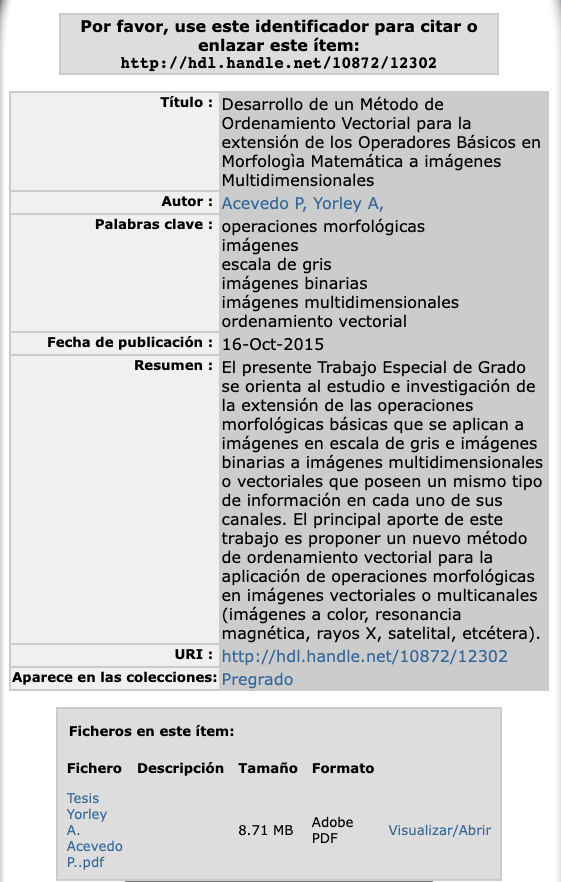
\includegraphics[width=0.6\linewidth]{images/01-intro/ficha_registro} 

}

\caption{Modelo de ficha registro en Saber UCV}\label{fig:ficharegistro}
\end{figure}

Con los textos \textbf{Resumen}, con la \textbf{fecha}, el \textbf{nombre del autor}, las \textbf{palabras claves} de todos los trabajos catalogados como Tesis en el repositorio Saber UCV es con los que se conformará el \textbf{\emph{Corpus}}.

Para el momento en que se presenta esta Investigación bajo la categoría \textbf{Tesis} reposan 10.481 documentos distribuidos con las jerarquías que se muestran en el cuadro \ref{tab:jerarquias}.

\providecommand{\docline}[3]{\noalign{\global\setlength{\arrayrulewidth}{#1}}\arrayrulecolor[HTML]{#2}\cline{#3}}

\setlength{\tabcolsep}{2pt}

\renewcommand*{\arraystretch}{1.5}

\begin{longtable}[c]{|p{1.06in}|p{0.95in}}

\caption{Total documentos por jerarquía
}\label{tab:jerarquias}\\

\hhline{>{\arrayrulecolor[HTML]{666666}\global\arrayrulewidth=2pt}->{\arrayrulecolor[HTML]{666666}\global\arrayrulewidth=2pt}-}

\multicolumn{1}{!{\color[HTML]{000000}\vrule width 0pt}>{\raggedright}p{\dimexpr 1.06in+0\tabcolsep+0\arrayrulewidth}}{\fontsize{11}{11}\selectfont{\textcolor[HTML]{000000}{\global\setmainfont{DejaVu Sans}{jerarquía}}}} & \multicolumn{1}{!{\color[HTML]{000000}\vrule width 0pt}>{\raggedleft}p{\dimexpr 0.95in+0\tabcolsep+0\arrayrulewidth}!{\color[HTML]{000000}\vrule width 0pt}}{\fontsize{11}{11}\selectfont{\textcolor[HTML]{000000}{\global\setmainfont{DejaVu Sans}{cantidad}}}} \\

\hhline{>{\arrayrulecolor[HTML]{666666}\global\arrayrulewidth=2pt}->{\arrayrulecolor[HTML]{666666}\global\arrayrulewidth=2pt}-}

\endfirsthead

\hhline{>{\arrayrulecolor[HTML]{666666}\global\arrayrulewidth=2pt}->{\arrayrulecolor[HTML]{666666}\global\arrayrulewidth=2pt}-}

\multicolumn{1}{!{\color[HTML]{000000}\vrule width 0pt}>{\raggedright}p{\dimexpr 1.06in+0\tabcolsep+0\arrayrulewidth}}{\fontsize{11}{11}\selectfont{\textcolor[HTML]{000000}{\global\setmainfont{DejaVu Sans}{jerarquía}}}} & \multicolumn{1}{!{\color[HTML]{000000}\vrule width 0pt}>{\raggedleft}p{\dimexpr 0.95in+0\tabcolsep+0\arrayrulewidth}!{\color[HTML]{000000}\vrule width 0pt}}{\fontsize{11}{11}\selectfont{\textcolor[HTML]{000000}{\global\setmainfont{DejaVu Sans}{cantidad}}}} \\

\hhline{>{\arrayrulecolor[HTML]{666666}\global\arrayrulewidth=2pt}->{\arrayrulecolor[HTML]{666666}\global\arrayrulewidth=2pt}-}\endhead



\multicolumn{1}{!{\color[HTML]{000000}\vrule width 0pt}>{\raggedright}p{\dimexpr 1.06in+0\tabcolsep+0\arrayrulewidth}}{\fontsize{11}{11}\selectfont{\textcolor[HTML]{000000}{\global\setmainfont{DejaVu Sans}{doctorado}}}} & \multicolumn{1}{!{\color[HTML]{000000}\vrule width 0pt}>{\raggedleft}p{\dimexpr 0.95in+0\tabcolsep+0\arrayrulewidth}!{\color[HTML]{000000}\vrule width 0pt}}{\fontsize{11}{11}\selectfont{\textcolor[HTML]{000000}{\global\setmainfont{DejaVu Sans}{305}}}} \\





\multicolumn{1}{!{\color[HTML]{000000}\vrule width 0pt}>{\raggedright}p{\dimexpr 1.06in+0\tabcolsep+0\arrayrulewidth}}{\fontsize{11}{11}\selectfont{\textcolor[HTML]{000000}{\global\setmainfont{DejaVu Sans}{maestría}}}} & \multicolumn{1}{!{\color[HTML]{000000}\vrule width 0pt}>{\raggedleft}p{\dimexpr 0.95in+0\tabcolsep+0\arrayrulewidth}!{\color[HTML]{000000}\vrule width 0pt}}{\fontsize{11}{11}\selectfont{\textcolor[HTML]{000000}{\global\setmainfont{DejaVu Sans}{729}}}} \\





\multicolumn{1}{!{\color[HTML]{000000}\vrule width 0pt}>{\raggedright}p{\dimexpr 1.06in+0\tabcolsep+0\arrayrulewidth}}{\fontsize{11}{11}\selectfont{\textcolor[HTML]{000000}{\global\setmainfont{DejaVu Sans}{otras}}}} & \multicolumn{1}{!{\color[HTML]{000000}\vrule width 0pt}>{\raggedleft}p{\dimexpr 0.95in+0\tabcolsep+0\arrayrulewidth}!{\color[HTML]{000000}\vrule width 0pt}}{\fontsize{11}{11}\selectfont{\textcolor[HTML]{000000}{\global\setmainfont{DejaVu Sans}{1.239}}}} \\





\multicolumn{1}{!{\color[HTML]{000000}\vrule width 0pt}>{\raggedright}p{\dimexpr 1.06in+0\tabcolsep+0\arrayrulewidth}}{\fontsize{11}{11}\selectfont{\textcolor[HTML]{000000}{\global\setmainfont{DejaVu Sans}{pregrado}}}} & \multicolumn{1}{!{\color[HTML]{000000}\vrule width 0pt}>{\raggedleft}p{\dimexpr 0.95in+0\tabcolsep+0\arrayrulewidth}!{\color[HTML]{000000}\vrule width 0pt}}{\fontsize{11}{11}\selectfont{\textcolor[HTML]{000000}{\global\setmainfont{DejaVu Sans}{8.208}}}} \\





\multicolumn{1}{!{\color[HTML]{000000}\vrule width 0pt}>{\raggedright}p{\dimexpr 1.06in+0\tabcolsep+0\arrayrulewidth}}{\fontsize{11}{11}\selectfont{\textcolor[HTML]{000000}{\global\setmainfont{DejaVu Sans}{\textbf{Total}}}}} & \multicolumn{1}{!{\color[HTML]{000000}\vrule width 0pt}>{\raggedleft}p{\dimexpr 0.95in+0\tabcolsep+0\arrayrulewidth}!{\color[HTML]{000000}\vrule width 0pt}}{\fontsize{11}{11}\selectfont{\textcolor[HTML]{000000}{\global\setmainfont{DejaVu Sans}{\textbf{10.481}}}}} \\

\hhline{>{\arrayrulecolor[HTML]{666666}\global\arrayrulewidth=2pt}->{\arrayrulecolor[HTML]{666666}\global\arrayrulewidth=2pt}-}



\end{longtable}

La disponibilidad de trabajos en el repositorio por fecha de creación la presentamos en el histograma que se muestra en la figura \ref{fig:anos} .

\begin{figure}

{\centering 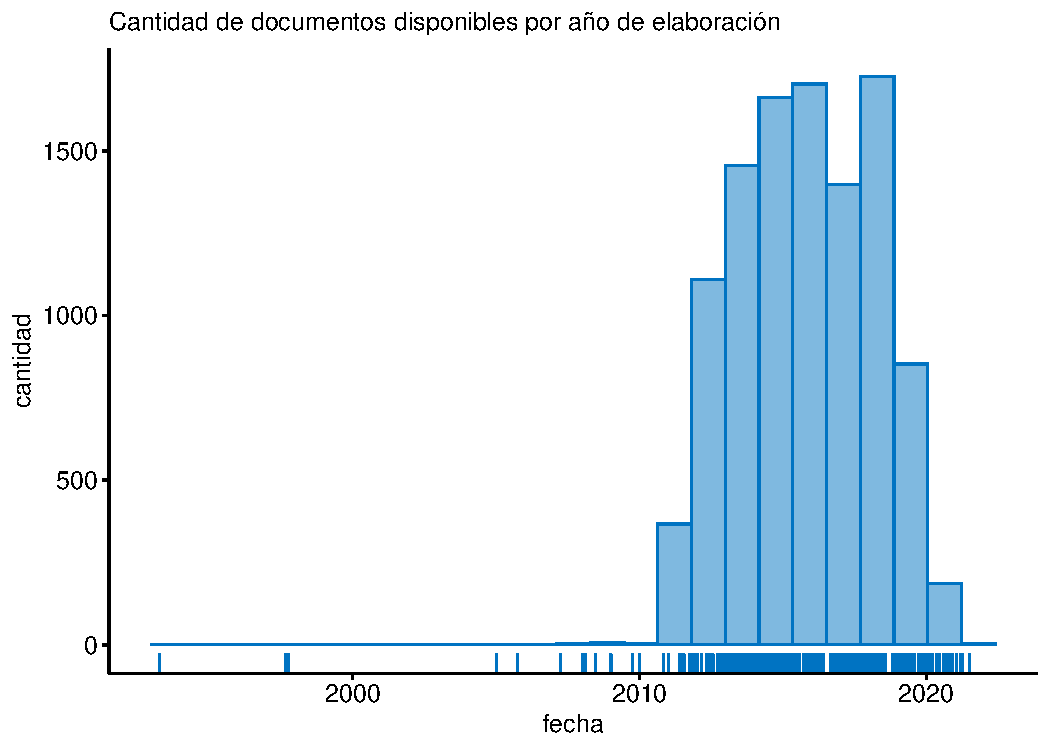
\includegraphics[width=0.6\linewidth]{_main_files/figure-latex/anos-1} 

}

\caption{Cantidad de documentos disponibles por año de elaboración}\label{fig:anos}
\end{figure}

Analizando la distribución de la frecuencia de la figura \ref{fig:anos} por año en que fue generada la investigación es necesario destacar que en el repositorio no se encuentran todas las investigaciones que se han realizado en la historia de la U.C.V. Actualmente se tienen incorporados solo 20 trabajos creados entre 1993 y 2011, siendo a partir de este último año cuando se empieza a realizar la ingesta de forma periódica y en mayor volumen. No obstante también queremos resaltar que desde el 2011 no se encuentran incorporados todos los trabajos generados dentro de la comunidad. Las razones que explican las omisiones o retardos en las incorporaciones queda fuera de los objetivos de este trabajo investigarlas.

\hypertarget{archivos-complementarios}{%
\subsubsection{Archivos complementarios:}\label{archivos-complementarios}}

Por razones que se expondrán en \ref{clasificacion} igualmente será necesario trabajar con los documentos anexos que indicamos en \ref{corpus} que disponen un vínculo de descarga en cada ficha \emph{HTML}. La descarga y el procesamiento de estos textos será necesario para complementar el corpus descrito en \ref{corpus}.

\hypertarget{requerimiento}{%
\section{Requerimiento inicial:}\label{requerimiento}}

Originalmente en la materia \emph{Tópicos Especiales en Sistemas de Información y Gerencia} se hizo un requerimiento para con los trabajos especiales de grado realizados por los alumnos de la Facultad de Ciencias, disponibles en Saber UCV, se hicieran \emph{Mapas de Conocimiento}.

Estos Mapas en un trabajo de \citep{dueñas2011} se definen como ``una metodología que busca encontrar palabras claves como unidad de análisis que permitan establecer cómo se relacionan diferentes campos científicos alrededor de un tema determinado''.

Ante esto se buscaron las estrategias que pudiesen satisfacer el requerimiento. Lo primero que se necesitaba era conformar el conjunto de datos, ya que no fue entregado como insumo.

Al realizar la descarga de los documentos con un \emph{web crawler} de diseño propio se pudo apreciar que no era viable separar los documentos de la Facultad de Ciencias al no existir ninguna etiqueta para realizar la selección.

Esto derivó en que fuese necesario diseñar una solución para clasificar los documentos previo a poder generar los Mapas de Conocimiento. En \ref{clasificacion} se expone con mayor detalle este problema.

\hypertarget{problema}{%
\section{Planteamiento del Problema:}\label{problema}}

El repositorio SABER UCV permite realizar búsqueda de documentos mediante procesos de recuperación de información, no obstante hay algunas características que pueden ser complementadas y mejoradas. A continuación se listan.

\hypertarget{clasificacion}{%
\subsection{I. No se posee clasificación de los documentos:}\label{clasificacion}}

El \textbf{\emph{Corpus}} que reposa en Saber UCV para ninguno de los documentos posee la etiqueta que clasifique a cual postgrado o carrera de pregrado pertenece. En caso de realizar una búsqueda y querer delimitarla a documentos que se circunscriban a una determinada área de conocimiento, actualmente es imposible y por ende resulta inviable evaluar la escuela o el postgrado y la facultad donde se hizo la investigación.

Tampoco se dispone de un listado con las etiquetas candidatas a asignar a cada uno de los documentos. Según lo investigado no es de conocimiento público un único directorio que contenga los nombres de las carreras de pregrado y de los distintos postgrados, significando esto que es un doble proceso de construcción el que se necesita hacer para realizar la clasificación de los documentos.

Relativo a este problema también surge el determinar cómo se realizará la comparación de cada una de las etiquetas con el texto de cada documento, incluso en detectar dónde se localiza el texto con el cual se efectuará la comparación, ya que el texto denominado \textbf{Resumen}, que vimos en la figura \ref{fig:ficharegistro}, no contiene la información necesaria para extraer dónde fue realizada la investigación (escuela o postgrado), haciendo necesario que sean analizados los documentos anexos a cada ficha que es propiamente el archivo, o los archivos, que componen cada una de las investigaciones.

En detalle, se tendrán que consolidar los archivos disponibles para cada investigación, los cuales no necesariamente se encuentran ordenados, por ejemplo por capítulo. Una vez realizada la consolidación se procederá a crear un archivo en texto plano. En algunos casos los documentos no contendrán texto sino imágenes del texto motivando que se tenga que realizar lectura OCR \footnote{OCR: ``\emph{optical character recognition}'' traducido como reconocimiento óptico de caracteres} para extraer el texto.

En este proceso de clasificación también se presentarán otros problemas relativos a los sistemas de codificaciones de los archivos \emph{file encodings} y a la introducción de caracteres no deseados dentro del texto, lo que será expuesto a detalle en el capítulo que contiene el desarrollo de la propuesta.

\hypertarget{p2}{%
\subsection{\texorpdfstring{II. Problemas en los resultados que generan los \textbf{\emph{Querys}}:}{II. Problemas en los resultados que generan los Querys:}}\label{p2}}

Existe un tipo de \emph{query} denominado \emph{``Full Text Search''} o búsqueda de texto completo que es donde se manifiesta una de las principales deficiencias que posee el Sistema Saber UCV. Aunque en él se pueden ejecutar búsquedas de texto, los métodos con los que se implementan estas búsquedas llevan a que sean generados una gran cantidad de resultados, en especial al usar más de una palabra en la búsqueda, presumimos que por usar el operador lógico \emph{OR} entre cada una de las palabras solicitadas en el \emph{query}.

\hypertarget{query}{%
\subsubsection{\texorpdfstring{Ejemplo \textbf{\emph{Query}} en Saber UCV:}{Ejemplo Query en Saber UCV:}}\label{query}}

Evaluemos el problema descrito con un ejemplo. Supongamos que queremos ver en el sistema Saber UCV los trabajos que un autor de nombre ``Jesús Fajardo'' ha realizado.

\begin{figure}

{\centering 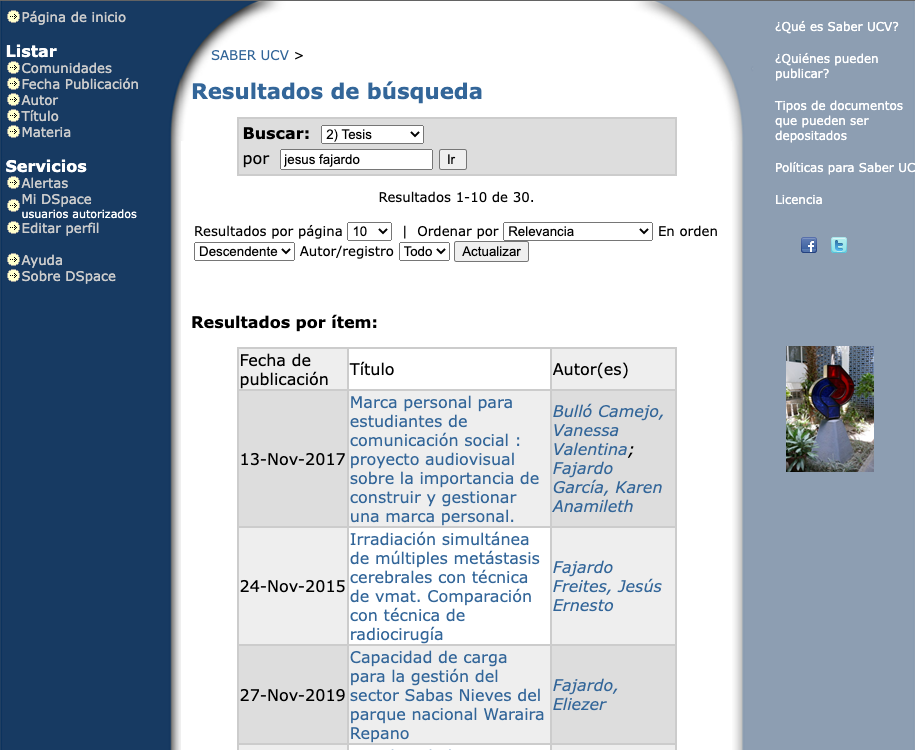
\includegraphics[width=0.6\linewidth]{images/01-intro/jesus_saber} 

}

\caption{Búsqueda de un autor "Jesus Fajardo" en www.saber.ucv.ve}\label{fig:busquedasaber}
\end{figure}

Al revisar los resultados que se muestran en la figura \ref{fig:busquedasaber} podemos apreciar que la primera posición de los 30 resultados que fueron encontrados, no muestra un autor que se llame ``Jesús Fajardo'' sino el apellido Fajardo. Incluso, al realizar la consulta del vínculo del primer resultado tampoco aparece la palabra ``Jesús'' dentro de todos los datos que muestra la ficha. Al revisar el segundo resultado vemos que sí coincide con el término que se estaba buscando, pero de resto ningún otro de los 28 resultados incluyen un ``Jesús Fajardo'' o un ``Jesús''.

Revisemos otro ejemplo de búsqueda esta vez con cuatro palabras que son ``simultánea de múltiples metástasis'' las cuales se encuentran en el título del trabajo visto anteriormente en la posición número dos. El resultado del \emph{query} lo podemos ver en la figura \ref{fig:busquedasaber2}.

\begin{figure}

{\centering 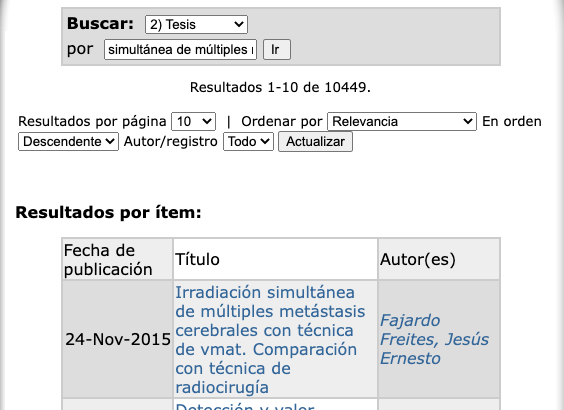
\includegraphics[width=0.6\linewidth]{images/01-intro/texto_saber} 

}

\caption{Búsqueda de "simultánea de múltiples metástasis" en www.saber.ucv.ve}\label{fig:busquedasaber2}
\end{figure}

La cantidad de resultados asciende a 10.449, cifra similar a la cantidad total de trabajos de la categoría ``Tesis'' que se encuentran en el repositorio, ya que como fue explicado anteriormente el Sistema Saber UCV debe aplicar el operador lógico \emph{OR} entre cada una de las palabras al momento de generar el \emph{query}. A manera de referencia podemos explicar que si hubiésemos querido realizar la búsqueda exacta de la frase, con haberle colocado comillas al inicio y al final obtendríamos la referencia al trabajo que previamente sabemos que es el que queremos encontrar.

Sin embargo, el uso de comillas para buscar una frase exacta genera una compensación entre la precisión en la búsqueda, lo cual se motiva en que al ser exacta, se cierra el umbral para encontrar otros resultados que pudiesen resultar de interés, así que el uso de este método puede presentar considerables desventajas.

Posterior a evaluaciones realizadas sobre el comportamiento de Saber UCV presumimos que los textos al ser procesados para su estructuración e ingesta en la base de datos no le son aplicadas técnicas con el algoritmo de Porter que permite realizar la extracción de la raíz o (\textbf{\emph{stemming}}) \footnote{proceso heurístico que remueve letras al final de las palabras con el objetivo de encontrar la raíz de la misma.} de cada una de las palabras. La importancia de aplicar este procesamiento será explicado en \ref{steaming}.

\hypertarget{antecedentes}{%
\section{Antecedentes:}\label{antecedentes}}

Se hizo una revisión bibliográfica de trabajos producidos dentro de la Universidad Central de Venezuela que puedan haber realizado investigaciones similares o complementarias a la que proponemos en este desarrollo. De particular interés resultó la ``Elaboración de un prototipo de buscador de documentos académicos de la Facultad de Ciencias'' \citep{Sánchez2008}, que fue una investigación que implementó el motor de búsqueda y repositorio denominado \textbf{BUSCONEST 1} que sirve exclusivamente a los documentos de investigación generados en la Facultad de Ciencias de la U.C.V. Este sistema sí cuenta con los trabajos clasificados por área del conocimiento donde fueron generados, no por contar con una rutina para la clasificación o por disponer de una etiqueta, sino por ser otra la fuente de los datos, en este caso el sistema de datos de la Biblioteca de la Facultad de Ciencias. Con lo analizado se comprende que no se resuelve el problema de clasificar el resto de documentos que reposan en Saber UCV.

Posteriormente \citep{guevara2015} presenta otra propuesta de motor de búsqueda con una versión modificada de BUSCONEST 1, denominada BUSCONEST 2, no obstante sólo se basa sobre textos producidos en la Facultad de Ciencias y en ninguno de estos desarrollos se realizan procesos de minería de texto.

Otra investigación que podemos señalar es ``Sistema de recomendación para el Buscador Académico Venezolano'' \citep{rodríguezlaguna2016}. En ella se señalan algunos repositorios digitales institucionales que se encuentran en Venezuela y se hace una propuesta de unificación de todos los contenidos y así poder generar recomendaciones de investigaciones a partir de una determinada búsqueda.

Evaluando estos antecedentes consideramos que nuestra propuesta resuelve el problema de la clasificación de documentos y permite efectuar las búsquedas sobre todo el conjunto de textos, así que podemos tener en perspectiva que nuestro desarrollo no solapará las propuestas mencionadas y generará un valor agregado favoreciendo a la actividad de investigación.

\hypertarget{estructura}{%
\section{Estructura del Trabajo:}\label{estructura}}

Este trabajo está estructurado de la siguiente forma: en un Capítulo 2 se expone el Marco Teórico. En el Capítulo 3 se describirá la propuesta técnica, el objetivo general y específicos de la Solución.

Tentativamente se propone que en el Proyecto de Trabajo de Grado en el Capítulo 4 se exponga el proceso de desarrollo de la Solución y las distintas pruebas que se realizaron para elegir una determinada tecnología por sobre otras, así como los resultados obtenidos, mientras que en el Capítulo 5 se presentarán las conclusiones y recomendaciones, posterior a la implementación del Sistema.

\hypertarget{teorico}{%
\chapter{Marco teórico-referencial:}\label{teorico}}

En este Capítulo se muestra el marco teórico en que se sustentan los aspectos de mayor relevancia para el desarrollo de la Solución. Principalmente se enuncian una serie de conceptos que involucran algoritmos de búsqueda, la recuperación de información, la minería de texto, el procesamiento del lenguaje natural, la estructuración de la base de datos y lo referente a la arquitectura distribuida en que se soporta la SSCSU.

\hypertarget{alghist}{%
\section{Reseña histórica:}\label{alghist}}

El profesor Donald Knuth señala, dentro del campo de las ciencias de la computación, que la \textbf{búsqueda} \emph{es el proceso de recolectar información que se encuentra en la memoria del computador de la forma más rápida posible, esto cuando tenemos una cantidad N de registros y nuestro problema es encontrar el registro apropiado de acuerdo a un criterio de búsqueda} \citep{knuth1997} (p.~392) .

Iniciamos con esta cita porque la recuperación de información gira en torno a un problema central de las ciencias de la computación que es la \textbf{búsqueda}. A continuación mencionaremos una serie de algoritmos que abordan este problema, no necesariamente resultando óptimos para dar solución a lo planteado en \ref{p2}.

En la década de 1940 cuando aparecieron las computadoras, las búsquedas no representaban mayor problema debido a que estas máquinas disponían de poca memoria \emph{RAM} pudiendo almacenar sólo moderadas cantidades de datos. Ellas estaban diseñadas para realizar cómputos y arrojar los resultados más no para tenerlos almacenados en memoria.

No obstante con el desarrollo del almacenamiento en memoria \emph{RAM} o en dispositivos de almacenamiento permanentemente, ya en la década de 1950 empezaron a aparecer los problemas de \textbf{búsqueda} y los primeras investigaciones para afrontarla. En la década de 1960 se adoptan por ejemplo estrategias basadas en arboles.

Los primeros algoritmos que sirvieron para localizar la aparición de una frase dentro de un texto, o expresado de forma más abstracta, como la detección de una subcadena \emph{P} dentro de otra cadena \emph{T}, fueron los algoritmos de \emph{Pattern-Matching} \citep{goodrich2013} (p.~584).

Así nos encontramos en la literatura con el algoritmo \emph{Fuerza Bruta} donde dado un texto T y una subcadena P, se va recorriendo cada elemento de la cadena T para detectar la aparición de la subcadena P. Si bien este algoritmo no presentaba el mejor desempeño, por contar con ciclos anestados en su ejecución, creó una forma válida de enfrentar el problema de la búsqueda de subcadenas de texto.

El algoritmo \emph{Knuth-Morris-Pratt} que se introdujo en 1976 tenía como novedad que se agregó una función que iba almacenando ``previas coincidencias parciales'' en lo que eran fallos previos y así al realizar un desplazamiento tomaba en cuenta cuántos caracteres se podían reusar. De esta forma se logró considerablemente mejorar el rendimiento en los tiempos de ejecución de \emph{O(n+m)} que son asintóticamente óptimos.

Posteriormente en 1977 el problema se enfrenta con un nuevo algoritmo que es el de \emph{Boyer-Moore} en el cual se implementan dos heurísticas (\emph{looking-glass y} \emph{character-Jump)} que permiten ir realizando algunos saltos en la búsqueda, ante la no coincidencia de la subcadena con la cadena y adicionalmente, el orden en el que se va realizando la comparación se invierte. Estas modificaciones permitieron obtener un mejor desempeño.

Sobre una modificación al algoritmo \emph{Boyer-Moore} se sustenta la utilidad \emph{grep} de la línea de comandos UNIX que igualmente le da soporte a diversos lenguajes que la usan para ejecutar búsquedas de texto con un proceso que comúnmente es conocido como \emph{grepping}. Esta utilidad fue ampliamente usada para resolver parcialmente lo expuesto en \ref{clasificacion}.

Los algoritmos mencionados anteriormente pueden ser usados en procesos de recuperación de información en conjunto con técnicas que pueden mejorar considerablemente los tiempos en la ejecución de las rutinas siendo una de estas el preprocesamiento de los textos, \emph{eg}. remover determinados caracteres, aplicar el algoritmo de porter, entre otras más.

Una estrategia que surgió para enfrentar las búsquedas de texto, fue el uso de la programación lineal donde bajo la premisa \emph{divida et impera} los problemas que requieren tiempo exponencial para ser resueltos son descompuestos en polinomios y por lo tanto se disminuye la complejidad en tiempo para ser resueltos. Entre este tipo de algoritmos podemos mencionar los de \emph{alineación del ADN .} Originalmente el algoritmo se desarrolló para resolver problemas de alineación de cadenas de ADN de forma parcial o total dentro de una cadena mayor. Posteriormente se identificó que este tipo de procedimiento era extrapolable a los subcadenas de texto. Una de las versiones de estos algoritmos es la denominada \textbf{\emph{Smith-Waterman}} que resultó de gran utilidad para resolver el problema planteado en \ref{clasificacion} ya que la estrategia de usar la utilidad \emph{grep} fue infructuosa en algunos casos.

Un gran paso para aproximarnos a la aparición de los Sistemas de Recuperación de Información lo representó el enfoque que presentan los algoritmos \emph{Tries}. Este nombre proviene del proceso de \emph{Information Retrieval} y principalmente se basa en hacer una serie de preprocesamientos a los textos para que al momento de ejecutar la búsqueda de texto, es decir, de la subcadena dentro de la cadena, ya tengamos una parte del trabajo realizado previamente y no tener que ejecutarlo todo \emph{``on the fly''}, es decir, sobre la marcha.

Un \emph{Trie} \citep{fredkin1960} es una estructura de datos que se crea para almacenar textos para así poder ejecutar más rápido la coincidencia en la búsqueda. En la propuesta de la SSCSU todos los textos van siendo procesados con distintas técnicas a medida que son insertados en la base de datos. Esto claramente representa una mejora en el desempeño con la disminución en los tiempos de búsqueda.

\hypertarget{infret}{%
\section{Recuperación de Información:}\label{infret}}

El eje central sobre el cual gira el proceso de recuperación de información (RI) es satisfacer las necesidades de información relevante que sean expresadas por un usuario mediante una consulta (\textbf{\emph{query}}) de texto. El investigador Charu Aggarwal en su libro sobre Minería de Texto \citep{miningt2012} (p.14) menciona que el objetivo del proceso de RI es conectar la información correcta, con los usuarios correctos en el momento correcto, mientras que otro de los autores con mayor dominio sobre el tema, Christopher Manning en su libro \emph{Information Retrieval} indica que ``es el proceso de encontrar materiales (generalmente documentos) de una naturaleza no estructurada (generalmente texto) que satisface una necesidad de información dentro de grandes colecciones (normalmente almacenada en computadores)'' \citep{manning2008} (p.~25).

Satisfacer una necesidad de recuperación de información no sólo se circunscribe a un problema \textbf{búsqueda} de un texto dentro de un \emph{corpus}. En la mayoría de los casos se deberá cumplir con ciertos criterios, o restricciones, como por ejemplo que el \emph{query} esté dentro de un período de fechas, o que se encuentre comprendido en un subconjunto del corpus que es a lo que se denomina \textbf{búsqueda múlti atributo}.

La información que se recolecte en una búsqueda tendrá distintos aspectos que aportarán peso en el orden en que sea presentada al usuario y no sólo vendrá dado por la aparición de las palabras sino también por otros elementos como lo puede ser la aparición de la frase del \textbf{\emph{query}} dentro del título, la proximidad (la cercanía entre dos palabras) que tengan los términos que conforman el \emph{query} o por otra parte la frecuencia que una palabra, o varias, se repitan dentro un determinado documento que compone el \emph{corpus}. Igual puede aportar un peso mayor a la recuperación de un documento las referencias (citas) que contengan otros documentos a ese determinado documento. El fin último será la extracción de los documentos que resulten de mayor relevancia para el usuario.

Incluso es válido incorporar documentos, en los resultados que arroje la búsqueda, que propiamente no coincidan con los términos buscados sino que contengan términos que sean sinónimos o también añadiendo a los resultados documentos que presenten alguna similitud con el texto del \textbf{\emph{query}}. Lo que acabamos de mencionar incorporará formalmente dentro del proceso de extracción de información algo de imprecisión con la intención última de enriquecer el proceso de \textbf{\emph{Information Retrieval}} \citep{kraft2017}.

Evaluando el proceso con cierto nivel de abstracción tenemos que el proceso de recuperación de información está compuesto principalmente por: un \emph{query}, por un corpus y por una función de \emph{ranking} para ordenar los documentos recuperados de mayor importancia a menor.

El desarrollo de los algoritmos expuestos en \ref{alghist} sumado a la necesidad de resolver los problemas asociados a la búsqueda de un texto dentro de un \emph{corpus} con múltiples atributos en tiempos aceptables y la abundante cantidad de información digital, potenciada por el uso generalizado de los computadores, abonó las condiciones para la creación de los \textbf{Sistemas de Recuperación de Información}.

\hypertarget{SRI}{%
\section{Sistemas de Recuperación de Información (SRI) :}\label{SRI}}

Los Sistemas de Recuperación de Información (\emph{Information Retrieval Systems-IRS}) son los dispositivo (software y/o hardware) que median entre un potencial usuario que requiere información y la colección de documentos que puede contener la información solicitada \citep{kraft2017} 1. El SRI se encargará de la representación, el almacenamiento y el acceso a los datos que estén estructurados y se tendrá presente que las búsquedas que sobre él recaigan tendrán distintos costos siendo uno de estos el tiempo que tarde en efectuarse.

Es de nuestro conocimiento que generalmente los datos estructurados son gestionados mediante un sistema de base de datos pero en el caso de los textos estos se gestionan por medio de un motor de búsqueda motivado a que los textos en un estado crudo carecen de estructura \citep{miningt2012} (p.~2). Son los motores de búsqueda (\emph{search engines}) los que permiten que un usuario pueda encontrar fácilmente la información que resulte de utilidad mediante un \emph{query}.

El SSCSU está diseñado como un IRS donde se pueden ejecutar querys que son procesados y los resultados que se obtienen son sometidos a una función de ranking que será expuesta en una fase posterior del desarrollo de esta investigación.

\hypertarget{ejemplos-de-irs}{%
\section{Ejemplos de IRS:}\label{ejemplos-de-irs}}

Profundizando en el tema de esta Investigación mencionaremos un par de páginas de internet que funcionan coomo IRS.

\begin{enumerate}
\def\labelenumi{\arabic{enumi}.}
\item
  Una es el proyecto denominado Arvix alojado en \url{https://arxiv.org/}, que es un repositorio de trabajos de investigación. Al momento del usuario hacer un requerimiento de información, adicional al texto de la búsqueda, se pueden indicar distintos filtros a aplicar como puede ser el área del conocimiento (física, matemática, computación, etc.). Igualmente se puede indicar si se quiere buscar sólo dentro del título de una investigación, o el autor, en el \emph{abstract, o} en las referencias, por ejemplo.

  Al ejecutar una búsqueda pueden ser recuperados miles de documentos y la interacción con el sistema permite ver que se genera un \emph{ranking} en la exhibición de los resultados obtenidos. El primero de estos \emph{rankings} se ordena con base en la fecha de publicación, pero es viable que se ordenaran los documentos por la relevancia que presentan.
\item
  También tenemos el portal de la Asociation Computery Machine (ACM) que incorpora motores de búsqueda con particulares características facilitando la labor de investigación y extracción de información ante una determinada necesidad. Esto lo decimos porque los resultados de una búsqueda son acompañados de distintas representaciones gráficas que le dan un valor adicional a la representación de los resultados. En la figura \ref{fig:busquedasacm} vemos una de estas representaciones que incluye la frecuencia de aparición del \emph{query} en el tiempo.
\end{enumerate}

\begin{figure}

{\centering 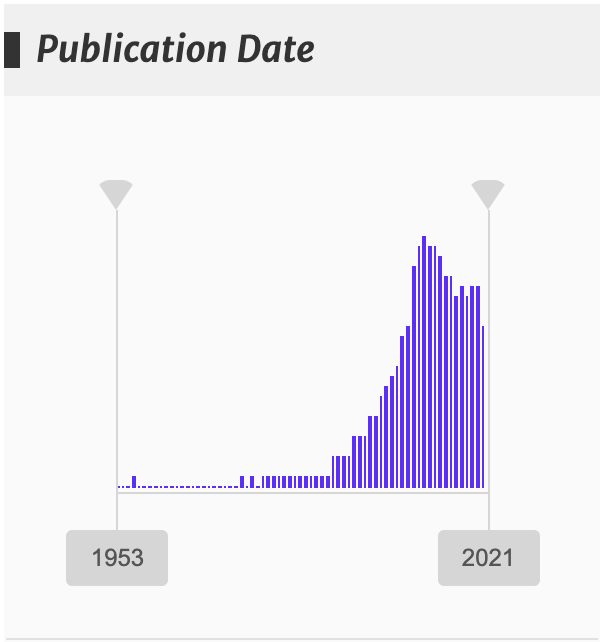
\includegraphics[width=0.4\linewidth]{images/02-marco-teorico/busquedaacm} 

}

\caption{Gráfico que acompaña resultados de búsqueda de un término en la biblioteca digital de la Association for Computing Machinery (https://dl.acm.org/)}\label{fig:busquedasacm}
\end{figure}

\hypertarget{modelos-de-recuperaciuxf3n-de-informaciuxf3n}{%
\section{Modelos de Recuperación de Información:}\label{modelos-de-recuperaciuxf3n-de-informaciuxf3n}}

\hypertarget{recuperaciuxf3n-boleana}{%
\subsection{Recuperación boleana:}\label{recuperaciuxf3n-boleana}}

Ante una búsqueda de información se recorre linealmente todo el documento para retornar un valor boleano indicando la presencia o no del término buscado. Es uno de los primeros modelos que se uso y está asociado a técnicas de \emph{grepping} \citep{manning2008} (p.3). El desarrollo de este modelo apareció entre 1960 y 1970.

El usuario final obtendrá como respuesta a su \emph{query} sólo aquellos textos que contengan el término. Es un modelo muy cercano a los típicos \emph{querys} de bases de datos con el uso de operadores ``AND'', ``OR'' y ``NOT''. En el procesamiento de los textos se genera una matriz de incidencia binaria término-documento, donde cada término que conforma el vocabulario, ocupa una fila \emph{i} de la matriz mientras que cada columna \emph{j} se asocia a un documento. La presencia de el término \emph{i} en el documento \emph{j} se denotará con un valor verdadero o un ``\textbf{1}''.

La recuperación boleana si bien representa una buena aproximación a la generación de \emph{querys} más rápidos, presenta una gran desventaja y es que al crecer la cantidad de documentos y el vocabulario, se obtiene una matriz dispersa de una alta dimensionalidad que hace poco efectiva su implementación.

Los documentos y los \emph{querys} son vistos como conjuntos de términos indexados, que luego fueron llamados ``bolsa de términos'' \emph{(bag of terms)}. Las deficiencias de este modelo recaen en que los resultados, no tienen ningún ranking. Si por ejemplo el término sobre el cual se realiza el \emph{query} aparece 100 veces en un documento y en otro aparece sólo una vez, en la presentación de los resultados ambos documentos aparecerán al mismo nivel, no pudiendo mostrar preferencia del uno sobre el otro.

Otra de las desventajas es que no se registra el contexto semántico de las palabras, incluso se pierde el orden en que aparecen las palabras en cada texto.

Este modelo se presume que en el cual se basa la implementación de Saber UCV y por eso es que en general se termina presentando el problema de que al usar el operador \emph{AND} en las búsquedas exactas mencionadas en \ref{query} se obtiene una alta \textbf{\emph{precision}} \footnote{Precision: la fracción, o porcentaje, de los documentos recuperados que son relevantes en la búsqueda efectuada.} en los resultados pero un bajo \textbf{\emph{recall}} \footnote{Recall: la fracción, o porcentaje, de los documentos relevantes en la colección que fueron recuperados por el sistema.} mientras que al usar el operador \emph{OR} da una baja \textbf{\emph{precisión}} y un gran \textbf{\emph{recall}}.

Con la propuesta del SSBSU se quiere una versión de recuperación de información que aplica métodos de mayor eficiencia, que permiten mejorar el desempeño (tiempo) y la calidad de los resultados.

\hypertarget{invind}{%
\subsection{Índices Invertidos:}\label{invind}}

Se denominan índices invertidos porque en vez de guardar los documentos con las palabras que en ellos aparecen, en estos se procede a guardar cada palabra y se indica los documentos en los cuales se encuentra y adicionalmente se puede registrar la posición en que aparece cada palabra con distintas granularidades, pudiendo ser estas: dentro del documento, del capítulo, del párrafo o de la oración. También pueden contener la frecuencia con que se presenta determinada palabra. Toda esta información nos permite mejorar los tiempos de búsqueda pero con ciertos costos.

El primero es el espacio en disco que implica guardar estos datos adicionales, que puede oscilar del 5\% al 100\% del valor inicial de almacenamiento, mientras que el segundo costo lo representa el esfuerzo computacional de actualizarlos una vez que se incorporan nuevos documentos \citep{Mahapatra2011}.

Existen diversos tipos de \textbf{Índices Invertidos} y constantemente se están realizando investigaciones que permitan mejorar su desempeño motivado en que sobre ellos recae gran parte de la efectividad que podamos obtener ejecutando los \emph{querys}. Algunos ejemplos de estos índices son el \emph{Generalized Inverted Index} (GIN), también está el RUM \footnote{En el vínculo \url{https://github.com/postgrespro/rum} se tiene acceso a la explicación e implementación de este índice para PostgreSQL.} o el VODKA \footnote{este índice fue presentado en la Postgres Conference en el año 2014 \url{https://www.pgcon.org/2014/schedule/attachments/318_pgcon-2014-vodka.pdf}}que es otra implementación con menos literatura sobre posibles usos pero con métodos disponibles para su uso en manejadores de base de datos como PostgreSQL.

El espacio que ocupa la implementación de estos índices se puede ver afectado, por un lado tenemos que se puede reducir mediante el preprocesamiento que hagamos a las palabras buscando su raiz con el stemming \{\#steaming\} o removiendo las stop words (las palabras que no generan mayor valor semántico como: la, el, tu).

Por otra parte el peso total se puede incrementar a medida que decidamos tener una granularidad más fina en el registro de las palabras y su ubicación dentro de los documentos. En el transcurso del desarrollo de nuestra investigación indicaremos en cuánto se incremento el espacio de almacenamiento en disco con la aplicación de este índice y la granularidad que se adoptó junto con el valor del costo en espacio de almacenamiento.

Continuando con los índices inversos hay estrategias que significan la adopción de generar dos índices inversos para un sistema, conteniendo uno de estos la lista de documentos y la frecuencia de la palabra, mientras que el otro registra la lista con las posiciones de la palabra.

El uso de los índices invertidos permite la denominada ``búsqueda de texto completa'' (\emph{full text search}) que es uno de los pilares que sustenta a los motores de búsqueda y se entiende por este tipo de búsqueda aquella que permite encontrar documentos que contienen las palabras claves o frases determinadas en el texto del \emph{query}. Adicionalmente podemos introducir el criterio de búsqueda de texto aproximado \emph{(approximate text searching)}, que permite flexibilizar la coincidencia entre el texto requerido y el resultado.

En la Solución que se propone, la optimización en la generación de este índice quedará bajo la administración del propio manejador de base de datos que es \emph{postgreSQL}.

Cuando la base de datos que registra el índice invertido crece y no es viable almacenarla en un único computador, es necesario acudir al uso de técnicas que permitan distribuir la base de datos con el uso de tecnologías como \emph{Spark, Hadoop, Apache Storm} entre otras.

\hypertarget{rank}{%
\subsection{Scoring Model:}\label{rank}}

Es un modelo aplicado en amplias colecciones de documentos donde es necesario exclusivamente mostrar al usuario que realizó la búsqueda, una fracción de los documentos encontrados, pero es necesario que estos sean los de mayor puntuación (\emph{score}), de acuerdo a distintos criterios que permitan determinar cuales son los que tienen mayor relevancia, como lo puede ser la cantidad de veces que se repite una palabra aparecida en el \emph{query} dentro del documento, o la distancia de aparición de cada una de las palabras que conforman el query (cantidad de palabras que median entre una y otra).

También se puede asignar un peso mayor en la generación del ranking, si una, o varias, de las palabras que generan el \emph{query} aparece dentro del título, o en otros campos que se registrasen en la base de datos.

\hypertarget{procesamientos-de-texto}{%
\section{Procesamientos de texto:}\label{procesamientos-de-texto}}

En esta sección mostramos métodos de trabajo con los textos. Para el idioma español no son de abundante literatura, a diferencia de aquellos que están en el idioma inglés. Incluso hasta hace unos pocos años las herramientas computacionales para el procesamiento de los textos \ref(nlproc) tampoco eran abundantes y sabiendo que son justamente los textos, el insumo que recibe de nuestro sistema de recuperación de información, la calidad en los procesamientos que sobre ellos hagamos, marcarán en gran medida la propia calidad del sistema que tengamos.

Como decíamos la literatura y herramientas disponibles para el NLP en el idioma español, fueron escasas durante un considerable período. Se tenían disponibles algunas como el coreNLP de la Universidad de Stanford pero no incluía todas las utilidades, tales como la identificación de parte del discurso \emph{(Part of Speech Tagging),} ni el análisis morfológico (\emph{Morphological Analysis)} o el reconocimiento de entidades nombradas (\emph{Named Entity Recognigtion)}, sino algunas pocas como el tokenizador \ref{token} y el separador de oraciones (Sentences Splitting).

Casos similares se presentaban con otras herramientas, siendo un caso aparte el esfuerzo del CLiC- Centre de Llenguatge i Computación quienes hicieron la anotación del Corpus AnCora \footnote{\textbf{AnCora} es un corpus del \textbf{catalán (AnCora-CA)} y del \textbf{español (AnCora-ES)} con diferentes niveles de anotación como lema y categoría morfológica, constituyentes y funciones sintácticas, estructura argumental y papeles temáticos, clase semántica verbal, tipo denotativo de los nombres deverbales, sentidos de WordNet nominales, entidades nombradas (NER), relaciones de correferencia (\url{http://clic.ub.edu/corpus/es/ancora})\[<http://clic.ub.edu/corpus/es/ancora>\]} . También la Universidad Politécnica de Cataluña creó la herramienta FreeLing \footnote{\url{https://nlp.lsi.upc.edu/freeling/node/1}} que permitió realizar algunas de las funcionalidades mencionadas en el párrafo anterior. No obstante su integración en cadenas de trabajo y la actualización de sus modelos de entrenamiento, presentan rezagos en comparación a otros modelos que actualmente se están usando, los cuales serán evaluados en el transcurso de esta investigación y serán señalados en un capítulo que aún está por desarrollar.

\hypertarget{nlproc}{%
\subsection{Procesamiento del Lenguaje Natural (natural language processing- NLP):}\label{nlproc}}

Son las técnicas computacionales desarrolladas para permitir al computador ``comprender'' el significado de los textos de lenguaje natural. En esta Investigación son aplicadas una serie de estos métodos sobre los textos que componen el Corpus y podemos mencionar las siguientes:

\hypertarget{token}{%
\subsubsection{Tokenizador:}\label{token}}

Básicamente es separar el documento en palabras, o unidades semánticas que tengan algún signficado a las cuales se le llaman \emph{tokens}. Para el idioma español no representa un mayor reto, ya que se puede usar el espacio como delimitador de palabras, no así en otros idiomas como el chino donde el problema se aborda de manera distinta.

Al obtener las palabras como entidades separadas de un texto nos permite calcular la frecuencia de uso de las mismas.

Es común que las librerías de procesamiento de lenguaje natural contengan tokenizadores que presentan un 100\% como métrica de precisión en el idioma español.

\hypertarget{ner}{%
\subsubsection{\texorpdfstring{Entidades Nombradas \emph{(named entity reconigtion-NER)}:}{Entidades Nombradas (named entity reconigtion-NER):}}\label{ner}}

Son los procesos que permiten la extracción de las distintas entidades contenidas dentro de los textos. Las entidades son: nombres, lugares, organizaciones. También permite detectar relaciones entre entidades. Las medidas de precisión en los módulos de NER alcanzan una medida cercana al 89\% en modelos entrenados con \emph{machine learning}, tal es el caso de spacy, que es una de las librerías propuestas para realizar estos procesamientos en nuestro desarrollo.

\hypertarget{pos}{%
\subsubsection{\texorpdfstring{Etiquetado de Partes del Discurso \emph{(Part of speech tagging-POS)}:}{Etiquetado de Partes del Discurso (Part of speech tagging-POS):}}\label{pos}}

Una de las técnicas usadas en el Procesamiento del Lenguaje Natural es el part-of-speech (POS) y consiste en asignar un rol sintáctico a cada palabra dentro de una frase \citep{eisenstein2019} siendo necesario para ello evaluar cómo cada palabra se relaciona con las otras que están contenidas en una oración y así se revela la estructura sintáctica.

Los roles sintácticos principales de interés en la elaboración de esta Investigación son los sustantivos, adjetivos y verbos.

\begin{itemize}
\item
  Los sustantivos tienden a describir entidades y conceptos.
\item
  Los verbos generalmente señalan eventos y acciones.
\item
  Los adjetivos describen propiedades de las entidades
\end{itemize}

Igualmente dentro del POS se identifican otros roles sintácticos como los adverbios, nombres propios, interjecciones entre otros.

El POS es un procesamiento que sirve de insumo para la coocurrencia de palabras, que es una de las formas en que se representan los resultados de los \emph{querys} en la SSCSU.

En el estado del arte este etiquetado alcanza un 98\% de precisión.

\hypertarget{steaming}{%
\subsubsection{Stemming:}\label{steaming}}

Es el proceso en que se consigue el lema de una palabra, entendiendo que el lema es la forma que por convenio se acepta como representante de todas las formas flexionadas de una misma palabra.

Al buscar el lema se tiene presente la función sintáctica que tiene la palabra, es decir que se evalúa el contexto en el que ocurre. Una de las ventajas de aplicar esta técnica es que se reduce el vocabulario del Corpus y eso conlleva a que también se reduce el espacio de búsqueda en los documentos.

En el estado del arte este etiquetado alcanza un 96\% de precisión.

\hypertarget{textmin}{%
\section{Minería de Texto:}\label{textmin}}

La extracción de ideas útiles derivadas de textos mediante la aplicación de algoritmos estadísticos y computacionales, se conoce con el nombre de minería de texto, analítica de texto o aprendizaje automático para textos (text mining, text analytics, machine learning from text). Se quiere con ella representar el conocimiento en una forma más abstracta y así poder detectar relaciones en los textos.

El uso de las técnicas de minería de texto ha ganado atención en recientes años motivado a las grandes cantidades de textos digitales que están disponibles. La minería de texto surge para dar respuesta a la necesidad de tener métodos y algoritmos que permitan procesar estos datos no estructurados \citep{miningt2012} . Una vez que mediante el proceso de recuperación de información tenemos un cúmulo de textos, es posible que necesitemos dar un paso más allá y usar un conjunto de técnicas que nos permitan analizar y digerir estos textos, mediante la detección de patrones.

Uno de los desafíos al trabajar con textos es darles estructura para que resulte viable trabajar con ellos desde la perspectiva de procesos computacionales.

Una de las primeras fases consiste en agrupar todos los textos en un Corpus. Posteriormente se procederá a conformar una matriz dispersa de una alta dimensionalidad que se denominará \emph{``Sparce Term-Document Matrix)} de tamaño \emph{n X d,} donde \emph{n} es el número total de documentos y \emph{d} es la cantidad de términos o vocabulario (palabras distintas) presentes entre todos los documentos. Formalmente sabemos que la entrada \emph{(i,j)} de nuestra matriz es la frecuencia (cantidad de veces que aparece) de la palabra \emph{j} en el documento \emph{i} .

El problema de la alta dimensionalidad de la matriz mencionada motiva ir aplicando otras técnicas que en principio puedan colaborar a reducirla por medio de simplificar los atributos, es decir, disminuyendo el vocabulario por ejemplo aplicando el algoritmo de Porter (stemming).

Igualmente a nivel de minería de texto se hace deseable poder contar con la identificación semántica de cada una de las palabras que conforman nuestro vocabulario, para así obtener representaciones que aportan un mayor significado. Los procesamientos inherentes al NLP mencionados anteriormente son insumo para la minería de texto.

\hypertarget{coocurrencia}{%
\subsection{Coocurrencia de Palabras:}\label{coocurrencia}}

En esta investigación se usará una técnica denominada ``Coocurrencia de Palabras'' para la detección de patrones en los textos. Esto consiste en evaluar las palabras que coocurren dentro de los documentos que conforman el \emph{corpus} y se puede hacer con distintas granularidades. Por ejemplo: las palabras que coocurren una seguida de otra o las que coocurren dentro de la misma oración, o dentro de un párrafo y así sucesivamente.

Para la representación visual se usan los grafos representando cada palabra un nodo y la coocurrencia de una palabra con otra implica que se extienda un arco entre ellas. Las palabras dispuestas para representarse en el grafo serán exclusivamente las que tengan la función dentro del discurso (POS) \ref{pos} de adjetivos y sustantivos, es decir que cada coocurrencia será un sustantivo con el adjetivo que la acompaña, donde es posible tener una relación de un sustantivo con \{0,1,\ldots,n\} adjetivos.

La selección de las funciones gramaticales propuestas se hace para disminuir el espacio de representación y se considera que los sustantivos, al contar con el adjetivo que las acompaña, logran hacer una representación que muestra proximidad semántica y se representan los temas (\emph{topics}) más relevantes \citep{segev2021}.

En el método que se usará en este Sistema se filtrarán las \emph{n} ( \emph{n} igual a 100 ), palabras que presenten mayor coocurrencia dentro de los resúmenes filtrados en el \textbf{\emph{query}}, siendo posible seleccionar la granularidad (todo el texto o en un párrafo).

En la figura \ref{fig:coocejem} podemos visualizar lo expuesto de una manera gráfica al ver la representación en un grafo de la coocurrencia de palabras sobre los textos de los resúmenes de las Tesis y TEG de la Escuela de Física de la U.C.V.

\begin{figure}

{\centering 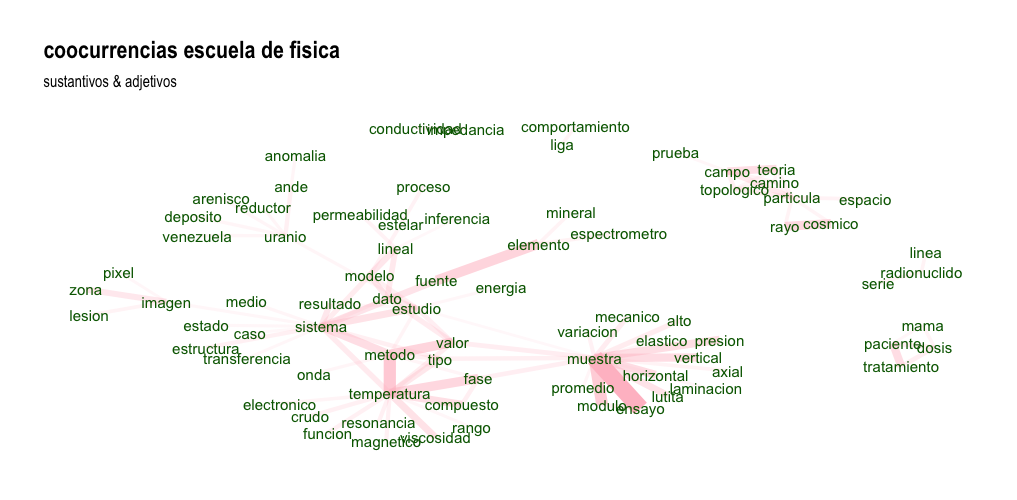
\includegraphics[width=0.9\linewidth]{images/02-marco-teorico/cooc} 

}

\caption{Coocurrencia de Palabras}\label{fig:coocejem}
\end{figure}

\hypertarget{similitud}{%
\section{Similitud de documentos:}\label{similitud}}

Para poder realizar la recomendación de documentos, una de las técnicas que se usa es medir la similitud que presenta un documento con los otros contenidos en el corpus. Un ejemplo de esta técnica es el uso de la similitud coseno que se explica con esta fórmula.

\begin{equation}
\cos ({\bf t},{\bf e})= {{\bf t} {\bf e} \over \|{\bf t}\| \|{\bf e}\|} = \frac{ \sum_{i=1}^{n}{{\bf t}_i{\bf e}_i} }{ \sqrt{\sum_{i=1}^{n}{({\bf t}_i)^2}} \sqrt{\sum_{i=1}^{n}{({\bf e}_i)^2}} }
\end{equation}

En la fórmula \emph{t} representa un documento y \emph{e} representa otro documento. Ambos documentos se asumen que están en un espacio con \emph{i} atributos, o dimensiones, y la intención es calcular un índice de similitud entre ambos documentos.

Este es uno de los métodos más usados para detectar similitudes en los textos, aunque existen otras fórmulas para el cálculo de la similitud como es el índice de jaccard.

El otro elemento de gran importancia en obtención de esta medición, es la representación que se haga del documento. Son distintas las técnicas que existen estando entre ellas la representación mediante ``bolsas de palabras'' o \emph{bag of words}. Recientemente se han creado formas más complejas para la representación como lo son los \emph{words embeddings} que son obtenidos mediante el entrenamiento de redes neuronales de aprendizaje profundo.

Estas formas de representación de textos serán investigadas más a fondo en futuras fases de la elaboración de este trabajo.

\hypertarget{sistemas-distribuidos}{%
\section{Sistemas Distribuidos:}\label{sistemas-distribuidos}}

Los distintos procesos y componentes de la Solución propuesta han sido diseñados e implementados como un sistema distribuido y por eso haremos una mención a este tema.

Una definición formal que se le puede dar a los sistemas distribuidos es ``cuando los componentes de hardware y/o sofware se encuentran localizados en una red de computadores y estos coordinan sus acciones sólo mediante el pase de mensajes'' \citep{distribu2012}.

Algunas de las principales características que tienen los sistemas distribuidos es la tolerancia a fallos, compartir recursos, concurrencia, ser escalables \citep{czaja2018} entre otras. Mencionamos estas en particular al ser propiedades que están presentes en la propuesta acá descrita.

\begin{enumerate}
\def\labelenumi{\arabic{enumi}.}
\item
  Fiabilidad o la llamada tolerancia a fallos: en caso de fallar un componente del sistema los otros se deben mantener en funcionamiento.
\item
  Compartir recursos: un conjunto de usuarios pueden compartir recursos como archivos o base de datos.
\item
  Concurrencia: poder ejecutar varios trabajos en simultáneo.
\item
  Escalable: al ser incrementada la escala del sistema se debe mantener en funcionamiento el sistema sin mayores contratiempos.
\end{enumerate}

\hypertarget{contenedores}{%
\subsection{Contenedores:}\label{contenedores}}

Un contenedor es una abstracción de una aplicación que se crea en un ambiente virtual, en el cual se encuentran ``empaquetados'' todos los componentes (sistema operativo, librerías, dependencias, etc.), que una aplicación necesita para poder ejecutarse. En su diseño se tiene presente que sean ligeros y que con otros contenedores pueden compartir el \emph{kernel}, usando un sistema de múltiples capas, que también pueden ser compartidas entre diversos contenedores, ahorrando espacio en disco del \emph{host} donde se alojan los contenedores.

El uso de los contenedores permite crear, distribuir y colocar en producción aplicaciones de software de una forma sencilla, segura y reproducible. También a cada contenedor se le puede realizar una asignación de recursos (memoria, cpu, almacenamiento) que garantice un óptimo funcionamiento de la aplicación que contienen.

Es importante señalar que el uso de esta tecnología añade un entorno de seguridad al estar cada contenedor en una ambiente isolado.

Para cada contenedor es necesario usar una imagen donde se definen las dependencias necesarias para su funcionamiento.

\hypertarget{orquestador}{%
\subsection{Orquestador:}\label{orquestador}}

Al tener diversos contenedores, donde cada uno aloja una aplicación distinta, puede resultar necesario que todos se integren en un sistema. Para que esta integración sea viable es necesario contar con un orquestador. Su uso permitirá lograr altos grados de portabilidad y reproducibilidad, pudiendo colocarlos en la nube o en centros de datos garantizando que se pueda hacer el \emph{deploy} de forma sencilla y fiel a lo que se implementó en el ambiente de desarrollo.

En el caso de la Solución propuesta se adoptará el uso de Docker Compose como orquestador y en el Capítulo que contiene la Propuesta Técnica \ref{propuestatec} serán expuestas las funcionalidades de cada contenedor y se apreciará la integración que brindará el orquestador.

\hypertarget{tendencias-actuales-sistemas-de-informaciuxf3n}{%
\section{Tendencias actuales Sistemas de Información:}\label{tendencias-actuales-sistemas-de-informaciuxf3n}}

Si bien anteriormente las búsquedas de información dentro de un conjunto de textos se procesaban determinando la aparición o no de palabras, o de frases dentro de un determinado texto, este método ha ido evolucionando para llegar hoy en día a un elevado nivel de abstracción, donde a partir de la necesidad de obtener una determinada información, es decir, de aquello que necesitamos buscar, que antes consistía en hacer \emph{match} con un objeto de información, hemos pasado de los motores de búsqueda ( \emph{search engines} ) a los motores de respuestas ( \emph{answering engines} ) \citep{balog2018}, donde el sistema ante un determinada consulta del usuario va a retornar una serie de resultados enriquecidos, mostrando la identificación de entidades, hechos y cualquier otro dato estructurado que esté de forma explícita, o incluso implícita, mencionado dentro de los textos que conforman el corpus.

Para lograr la generación de estos resultados se han tenido que conformar las llamadas bases de conocimiento o \emph{knowlodege bases}, que son repositorios donde previo a la búsqueda de la información dentro del sistema, se logra ir estructurando la organización de la información alrededor de objetos o datos específicos que se denominan \textbf{entidades}. Estos conceptos y métodos se asocian directamente a los que también se proponen, de manera más amplia, en la denominada \emph{web semántica} \footnote{Se basa en la idea de añadir \href{https://es.wikipedia.org/wiki/Metadato}{metadatos} \href{https://es.wikipedia.org/wiki/Sem\%C3\%A1ntica}{semánticos} y \href{https://es.wikipedia.org/wiki/Ontolog\%C3\%ADa_(Inform\%C3\%A1tica)}{ontológicos} a la \href{https://es.wikipedia.org/wiki/World_Wide_Web}{\emph{World Wide Web}}\emph{.} Esas informaciones adicionales ---que describen el contenido, el significado y la relación de los datos--- se deben proporcionar de manera formal, para que así sea posible evaluarlas automáticamente por máquinas de procesamiento. Tomado de \href{https://es.wikipedia.org/wiki/Web_sem\%C3\%A1ntica}{Wikipedia}} .

Como ejemplo de una \emph{knowledge bases} se puede mencionar a DBpedia, que se encuentra en la dirección \href{www.dbpedia.com}{www.www.dbpedia.org.com} y es un proyecto en donde puede acceder a una red global y unificada de grafos de conocimiento, la cual cubre más de 20 idiomas y principalmente genera sus grafos de conocimiento a partir de las publicaciones del Proyecto Wikipedia.

\hypertarget{temas-en-proceso-de-investigaciuxf3n}{%
\subsubsection{Temas en proceso de investigación:}\label{temas-en-proceso-de-investigaciuxf3n}}

Por estar aún en curso esta investigación a continuación se mencionan algunos temas que se está evaluando incluir en este marco teórico

\begin{itemize}
\item
  Métodos usados para el almacenamiento o la indexación como crear agrupamientos \emph{(clusters)} de aquellos documentos que compartan algunas características, por ejemplo, en la temática que aborden. Otra de las innovaciones que se están añadiendo a los sistemas de recuperación de información, es generar resúmenes con técnicas de procesamiento de lenguaje natural soportadas en el uso de arquitecturas de aprendizaje profundo \emph{(deep learning)} .
\item
  Resultados ante una búsqueda personalizados: al existir mecanismos como la sesión de usuario o las \emph{cookies} que guardan información contextual, permitiendo que ante un mismo \emph{query} en distintos equipos, los resultados sean distintos en función de la persona que hizo la búsqueda.
\item
  En cuanto al estado del arte existen distintas librerías y modelos de representación de documentos, palabras y caracteres. Algunos de estos modelos son fastext, word2vec, GPT3. Para este momento aún estamos haciendo la evaluación del uso de ellos para nuestra investigación, por lo cual, sólo los mencionamos referencialmente en este Antepryoecto.
\end{itemize}

\hypertarget{propuesta-tuxe9cnica}{%
\chapter{Propuesta Técnica:}\label{propuesta-tuxe9cnica}}

En este Capítulo se detalla la propuesta técnica de la Solución en la sección \ref{propuestatec}. Posteriormente se indica el Objetivo General \ref{objetivogral} y los Objetivos Específicos \ref{objetivosespe} que se aspiran cubrir en el desarrollo. A continuación se muestra el esquema general de la aplicación \ref{esquemas}, junto con el esquema de funcionamiento en los contenedores \ref{contenedores} y se describe el funcionamiento de cada contenedor.

Se realiza un análisis de factibilidad en la sección \ref{factibilidad} para la implementación y se muestra un cronograma \ref{cronograma} de actividades.

\hypertarget{propuestatec}{%
\section{Propuesta Técnica:}\label{propuestatec}}

Crear una Solución que funcione como una aplicación web distribuida bajo la arquitectura cliente-servidor. Del lado del servidor se encontrarán contenedores que alojarán los distintos servicios necesarios para el funcionamiento.

Del lado del cliente se podrán formular los \emph{querys} con múltiples atributos (la frase a buscar, la jerarquía académica, intervalo de fechas, facultad y/o escuela de adscripción).

La Solución permitirá generar procesos de extracción de información (\emph{information retrieval}) y los resultados se mostrarán en tablas interactivas, gráficos y grafos de coocurrencia de palabras. Adicionalmente se indicarán recomendaciones de textos basados en la similitud que presente un documento con los otros.

Los textos del resumen de cada tesis con los cuales se conformará el \emph{Corpus}, serán obtenidos y actualizados mediante técnicas de \emph{web crawling} realizadas al repositorio Saber UCV.

Se opta por la estrategia de hacer el \emph{web crawling} a los documentos contenidos en Saber UCV al no ser posible, al momento de realizar esta propuesta, la obtención de la base de datos de los documentos ahí alojados.

La Solución propuesta está diseñada para irse actualizando periódicamente incorporando los nuevos documentos que sean alojados en el repositorio Saber UCV.

Contará con un procedimiento que permite clasificar los documentos (tesis) por área académica, según donde haya efectuado estudios el autor del trabajo, al ser la tesis el requisito necesario para obtener el título de grado. Actualmente el repositorio Saber UCV no dispone de esta clasificación.

\hypertarget{objetivogral}{%
\section{Objetivo:}\label{objetivogral}}

Crear una Solución que permita realizar la clasificación de documentos y la búsqueda de información sobre los trabajos de investigación que se encuentran en el Repositorio SABER UCV usando técnicas de extracción de información (\emph{information retrieval}).

Para el procesamiento de las búsquedas será usado un sistema distribuido con distintos componentes (contenedores) que permitan la ingesta, procesamiento y transformación de los datos, al igual que el alojamiento de los mismos en una base de datos.

\hypertarget{objetivosespe}{%
\section{Objetivos Específicos}\label{objetivosespe}}

\begin{itemize}
\item
  \emph{Querys} multi atributo en distintas dimensiones: tiempo, jerarquías (pregrado, especializaciones, maestría y/o doctorado), facultad ,carreras o postgrados.
\item
  A cada resultado que arroje la búsqueda se le debe asignar un nivel de relevancia. El conjunto de los textos recuperados se debe mostrar ordenadamente de mayor a menor relevancia. La asignación de la relevancia será hecha mediante una función que cuente con distintos parámetros.
\item
  Los datos: textos, fechas, clasificaciones, y demás que sean necesarios para el funcionamiento de la Solución, deben registrarse en una base de datos estructurada y la ingesta y consulta se efectuará mediante un manejador de base de datos.
\item
  Generar recomendaciones de textos basados en la similitud coseno que presente un documento con cada uno de otros que conforman el \emph{Corpus}.
\item
  En los documentos extraídos se debe contar con el enlace a los documentos que reposan en Saber UCV.
\item
  Permitir la concurrencia de accesos al Sistema.
\item
  La tolerancia a fallas en los contenedores.
\item
  Contar con el certificado SSL para acceso seguro por parte de los visitantes.
\item
  Procesar las coocurrencias de las palabras más comunes las cuales se deberán visualizar mediante grafos.
\item
  Disponer de una aplicación web para el acceso al Sistema por parte del cliente.
\item
  Disponer de ventanas emergentes de ayuda en la interface gráfica de la aplicación web.
\item
  En la representación de coocurrencias de palabras mediante grafos, se debe poder filtrar documentos interactivamente al hacer \emph{click} con el \emph{mouse} sobre los arcos que unen un par de nodos, donde cada uno de estos representa la coocurrencia de una dupla de palabras. El \emph{click} generará el evento para el query sobre los documentos que contienen esa determinada coocurrencia.
\end{itemize}

\hypertarget{esquemas}{%
\section{Esquema del SSCSU:}\label{esquemas}}

Podemos representar el Sistema y sus interacciones mediante un esquema con un elevado grado de abstracción. Ver figura \ref{fig:esquema}.

\begin{figure}
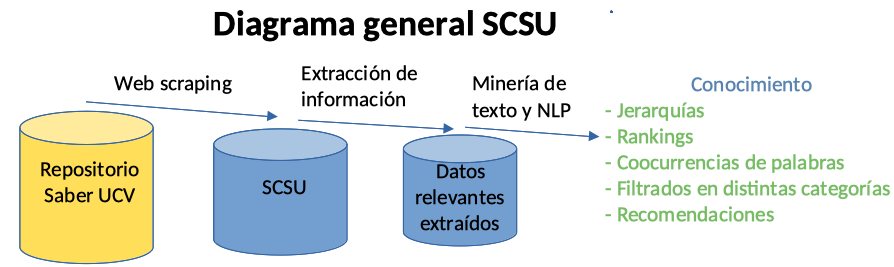
\includegraphics[width=1\linewidth]{formas/diagramageneral} \caption{Esquema General}\label{fig:esquema}
\end{figure}

En la figura \ref{fig:esquema} se muestra como el SSCSU está diseñado para que mediante técnicas de \emph{web crawling} se pueda extraer la información del repositorio Saber UCV. Posteriormente el sistema ante la consulta del usuario va a recuperar los documentos que sean relevantes, representando el conocimiento con la generación de jerarquías, rankings, coocurrencias de las palabras más mencionadas y recomendaciones de texto según similitudes.

El SSCSU se implementará mediante el uso de Docker. En la figura \ref{fig:esquemadocker} se muestra el esquema con los contenedores.

\begin{figure}
\includegraphics[width=0.9\linewidth]{formas/diagrama_docker1} \caption{Diagrama de Componentes}\label{fig:esquemadocker}
\end{figure}

\hypertarget{cliente---servidor}{%
\subsection{Cliente - Servidor:}\label{cliente---servidor}}

La arquitectura \textbf{cliente-servidor} en esta Propuesta se basa en:

\hypertarget{cliente---navegador-web}{%
\subsubsection{1 - Cliente - Navegador web:}\label{cliente---navegador-web}}

El acceso del cliente a la aplicación web se hace en el navegador web. Este realiza la petición al servidor que aloja la Solución. Actualmente se cuenta con un prototipo al que se puede acceder en la dirección \url{https://proyecta.me/}.

El sistema no está diseñado para usarse desde dispositivos móviles, aunque igualmente es viable el acceso no estando optimizada la interfaz del usuario ni las visualizaciones de los resultados de los \emph{querys}.

\hypertarget{servidor}{%
\subsubsection{2 - Servidor:}\label{servidor}}

El prototipo del sistema requiere para funcionar al menos estos recursos:

\begin{itemize}
\tightlist
\item
  2 CPU virtual
\item
  2 GB de memoria RAM
\item
  50 GB de disco duro
\end{itemize}

En el servidor se instala el software Docker sobre el cual se despliegan los siguientes contenedores:

\hypertarget{contenedores}{%
\subsection{Contenedores:}\label{contenedores}}

\hypertarget{docker-compose}{%
\subsubsection{Docker Compose:}\label{docker-compose}}

Funciona como un orquestador para correr aplicaciones distribuidas en múltiples contenedores usando un archivo en formato yml donde se establecen las imágenes, los puertos y los volúmenes que serán usados y compartidos por cada uno de los contenedores.

\hypertarget{contenedor-con-nginx}{%
\subsubsection{Contenedor con Nginx:}\label{contenedor-con-nginx}}

Es el servidor web/proxy inverso de código abierto que sirve para redireccionar las peticiones del puerto 80 al puerto 8090. Mediante este contenedor también se define el certificado SSL para permitir conexiones por el protocolo HTTPS.

Este contenedor fue generado desde una imagen oficial de NGINX que se encuentra en el \textbf{\emph{docker hub}} \footnote{repositorio de imágenes de contenedores de docker.} sin añadir ninguna capa (layer) adicional.

\hypertarget{contenedor-con-cerbot}{%
\subsubsection{Contenedor con Cerbot:}\label{contenedor-con-cerbot}}

Cerbot es una herramienta de código abierto que permite habilitar las conexiones mediante el protocolo HTTPS con el uso de un certificado ``Let´s Encrypt''. El uso de este certificado está asociado al uso de un dominio en el \emph{deploy} de la aplicación.

Este contenedor fue generado desde una imagen de CERBOT del \textbf{\emph{docker hub}} sin ninguna modificación posterior.

\hypertarget{conshinyproxy}{%
\subsubsection{Contenedor con Shinyproxy:}\label{conshinyproxy}}

Es una implementación del servidor ``\emph{Spring boo}t'' que dará servicio a las aplicación web desarrolladas en \emph{shiny} \footnote{Shiny un framework para crear aplicaciones web en el lenguaje de programación R.} \ref{conshiny}. Con el uso de este \emph{middleware} se obtienen las siguientes ventajas:

\begin{itemize}
\item
  Ante cada petición de acceso al servidor se despliega un \emph{workspace} completamente aislado, es decir, un contenedor distinto. Las aplicaciones desarrolladas en \emph{shiny} son \emph{single threaded} y adoptar esta estrategia representa una ventaja, motivado a que se pueden controlar los recursos de memoria y cpu asignados a cada contenedor que se despliega.
\item
  Permite establecer \emph{login} en el uso de la aplicación y grupos de usuarios. También da soporte a distintos métodos de autenticación. Si bien en estos momentos la aplicación es de libre acceso, en algún momento se pudiese restringir y no sería necesaria ninguna modificación en la arquitectura, más allá de cambiar el archivo de configuración.
\item
  Uso de una tecnología estable y probada.
\end{itemize}

Es necesario destacar que originalmente \emph{Shiny} como \emph{framework} cuenta con su propio software que actúa como servidor, pero para tener acceso a ciertas funcionalidades es necesario pagar por el servicio directamente a la Fundación RStudio Software y usar el alojamiento que ellos proveen, no siendo todos los componentes de código abierto. Por ejemplo, el acceso mediante \emph{login} no está disponible en la versión libre del \emph{Shiny Server} sino en la \emph{Shiny Server Professional}.

Ciertas configuraciones de librerías e incluso la propia contenerización de la aplicación, no es posible usando el servicio pago, así que la propuesta acá adoptada, si bien representa un mayor esfuerzo en la configuración, claramente implica que se obtienen una serie de ventajas, por todas las adaptaciones y control que es posible realizar al y sobre el sistema.

Este contenedor funciona en el puerto 2375 y fue generado desde la imagen del docker hub \emph{Shinyproxy} sin ninguna modificación.

\hypertarget{conshiny}{%
\subsubsection{\texorpdfstring{Contenedor con ``\emph{R Shiny Web App framework}'':}{Contenedor con ``R Shiny Web App framework'':}}\label{conshiny}}

En este contenedor es donde reposa la aplicación web con todas las librerías necesarias para generar las visualizaciones y remitir los \emph{querys} al contenedor del manejador de la base de datos \ref{conposgres} . Como comentamos anteriormente, cada vez que ocurre desde el navegador del cliente una petición de acceso, desde el contenedor \emph{shinyproxy} \ref{conshinyproxy}, se crea una replica de este contenedor con todos los elementos necesarios para que la app funcione correctamente.

En caso de presentar alguna falla, el sistema sería tolerante, porque se pueden seguir recibiendo peticiones que replicarían una imagen nueva del contenedor sin afectar al que presentase el fallo, o viceversa.

Desde este contenedor se realiza el acceso de lectura al contenedor que contiene \emph{PostgreSQL} \ref{conposgres} donde reposa la base de datos que contiene los textos ya procesados.

Por los momentos no hay escritura de datos en las tablas, pero está contemplado que se registren los querys formulados en alguna tabla, junto con los documentos que el usuario revisa mediante las interacciones, para así generar métricas de calidad del sistema y del uso que se le da.

La imagen que se usa en este servidor fue definida a medida con todos los recursos necesarios.

En un posterior Capítulo a desarrollar en donde se mostrará el proceso de desarrollo de la Solución, serán descritas todas las librerías que se encuentran incluidas en este contenedor y se expondrán las razones para seleccionar cada una de ellas.

Varios de los procesos que se ejecutan en este contenedor ocurren al momento de recibir un \emph{query,} no obstante todos los procesos que puedan ser pre computados, se trata de ejecutarlos previamente en el contenedor ``R Servicios'' \ref{conservicios}, para lograr así la disminución de los tiempos.

Funcionalidades principales: \textbf{ENTRADAS}

\begin{itemize}
\item
  Contiene un campo para la entrada de texto que generará el query.
\item
  Contiene un selector para indicar si se quiere generar la coocurrencia de palabras
\item
  Contiene tablas para seleccionar:

  \begin{enumerate}
  \def\labelenumi{\arabic{enumi})}
  \tightlist
  \item
    Nivel académico del trabajo. Opciones (pregrado, especialización, maestría, doctorado).
  \item
    Facultad o Centro de adscripción. Opciones: 11 Facultades más un centro (CENDES).
  \item
    Nombre del pregrado o postgrado. En total son 412 las opciones.
  \end{enumerate}

  Cada una de las tablas anteriores se actualiza según se vayan seleccionando las relaciones y la disponibilidades. Por ejemplo, al seleccionar pregrado solo se mostrarán los nombres de las carreras de pregrado, pero si se selecciona también el nombre de la Facultad, sólo se mostrarán las carreras de pregrado dentro de la Facultad seleccionada. Para una determinada tabla también se permiten selecciones múltiples dando una total flexibilidad al momento de ejecutar los \emph{querys}.
\end{itemize}

\textbf{SALIDAS} - Ante el \emph{query} se genera:

\begin{itemize}
\item
  Una tabla creada con la librería \emph{reactable}. En la misma se muestra cada uno de los documentos recuperados con los distintos atributos disponibles: autor, fecha, palabras claves, texto resumen. El orden en que aparece está generado con una función de ranking. Adicionalmente se muestra un enlace al repositorio Saber UCV que es donde se encuentra alojado el respectivo trabajo (el documento en PDF). Igualmente se presentan los textos que tienen mayor similitud con el texto seleccionado.
\item
  Un gráfico con la frecuencia por año de los trabajos extraídos mediante el \emph{query}. El gráfico se generá con la librería \emph{apexcharter} que es un wraper para Javascript, por lo cual el gráfico tiene ciertas interactividades. Con el \emph{hoover} muestra el valor de cada columna.
\item
  Gráfico de coocurrencia interactivo de palabras: se genera mediante la librería de \emph{VisNetwork} que también es un \emph{wrapper} de javascript. Este gráfico permite seleccionar un arco de unión entre dos palabras coocurrentes. Al realizar la selección se filtran un subconjunto de los documentos que contienen ambas palabras representadas por nodos. Los documentos filtrados se mostrarán en una tabla contigua, también generada en \emph{reactable}, donde sólo se incluye el texto resumen de cada trabajo. En un próximo Capítulo a desarrollar será mencionado el diseño y funcionamiento a detalle de esta visualización.
\item
  Gráfico de coocurrencia estático de palabras: mediante la librería \emph{ggraph} son generados un par de gráficos con distintas granularidades. El primero exhibe la misma coocurrencia de palabras expuesta en el punto anterior pero esta vez es generada en una visualización estática. En cuandoa la granularidad se muestran las palabras que coocurren dentro de todo el resumen, El segundo gráfico también muestra la coocurrencia, pero solo de palabras que coocurren una seguida de otra dentro del texto resumen, es decir que se muestran los resultados con una menor granularidad.
\end{itemize}

Con la librería \emph{UdPipe} se generan las estructuras de datos necesarias para generar los grafos (arcos y nodos).

\hypertarget{conposgres}{%
\subsubsection{Contenedor con PostgreSQL:}\label{conposgres}}

En este contenedor tenemos una imagen de \emph{PostgreSQL} versión 13.3. No fue realizada ninguna otra modificación distinta a la definición de usuarios y poblado desde base de datos incluyendo un volumen compartido para garantizar que tengamos ``datos persistentes. Este contenedor recibe consultas del contenedor''R Shiny Web App framework'' \ref{conshiny} y escritura desde el contenedor ``R imagen Servicios'' \ref{conservicios}.

En este contenedor ocurre la indexación de la base de datos y la generación del ranking al procesar el resultado con la función de PosgreSQL llamada tsrank \footnote{esta función mide la relevancia de los documentos para una consulta en particular, de modo que cuando haya muchas coincidencias, las más relevantes puedan mostrarse primero tomando en cuenta la información léxica, de proximidad y estructural del documento (título, cuerpo del documento, etc).}.

En una tabla se encuentra la identificación del documento, la fecha de creación y propiamente los textos que mediante el Tsvector \footnote{El Tsvector es una función de postgresql que crea una estructura de datos que es una lista ordenada de distintos lexemas, que son palabras que se han normalizado para fusionar diferentes variantes de la misma palabra mediante el algoritmo de Porter.} almacena el título, el resumen, el autor y las palabras claves.

En otra tabla se encuentra el almacenamiento del procesamiento que se le hace a los textos, clasificando cada una de las palabras mediante el \emph{part of speach} , y registrando el identificador del documento al que está asociada y el lema \footnote{El lema es la forma que por convenio se acepta como representante de todas las formas flexionadas de una misma palabra.}de cada una.

El TSvector es la estructura de datos que permite la búsqueda de texto completa (\emph{Full Text Seach}) mediante la función de \emph{PostgreSQL} denominada \emph{tsquery}. En un futuro capítulo a desarrollar será mostrado el diseño de las tablas con sus campos.

\hypertarget{conservicios}{%
\subsubsection{Contenedor con ``R Imagen Servicios'':}\label{conservicios}}

En este contenedor se creó una imagen con todos los servicios necesarios para realizar el web crawling, el procesamientos de textos y la descarga de los archivos desde Saber UCV para realizar la clasificación de las Tesis. Al iniciar el Sistema también contiene las funcionalidades que permiten realizar la creación de la base de datos, de las tablas y el poblado de estas.

Periodicamente es invocado este contenedor para realizar los procesos de incorporación de aquellos documentos nuevos que se detecte que están disponibles en Saber UCV.

En una primera fase se uso la utilidad del sistema operativo linux para la programación de actividades, sin embargo se está implementando el uso de la tecnología \emph{Apache Airflow} para la ejecución de la programación de los flujos de trabajo.

La imagen base usada es la del proyecto \textbf{\emph{Rocker}} \citep{RJ-2017-065:2017} ,la cual es una versión ampliamente probada y optimizada en, y por, la comunidad de usuarios de R.

Posteriormente serán descritas todas las librerías que fueron añadidas mediante una capa (layer) a este contenedor. Por los momentos podemos citar que se encuentran agregadas las siguientes:

\hypertarget{text-mining-y-nlp}{%
\paragraph{Text Mining y NLP:}\label{text-mining-y-nlp}}

Generalmente las distintas librerías que permiten realizar procesos de \emph{Natural Language Processing} también hacen procesos de \emph{Text Mining} parcial o totalmente. En la investigación fueron evaluadas múltiples librerías como \emph{Spacy, Quanteda, OPENLP, CoreNLP, Freeling y Udpipe}.

En una futura entrega se hará una breve mención a cada una y la razón por la cual se adoptó Spacy para varios de los procesos de NLP.

Para ejecutar \emph{Spacy} es necesario usar los archivos que se encuentran en el contenedor \emph{``Python Spacy''} , \ref{conspacy} donde está instalada la libraría \emph{Spacy} que corre en \emph{Python}.

Procesos que se ejecutan llamando al contenedor ``Python Spacy'': Tokenización, POS y Lematización.

También en este contenedor se realizan los siguientes procesos:

\begin{enumerate}
\def\labelenumi{\arabic{enumi}.}
\item
  Poblado base de datos: se hace el \emph{web crawling} para el poblado inicial y adicionales de la base de dato, con los textos de los Resúmenes.
\item
  Clasificación de los documentos: mediante una rutina compuesta por varios algoritmos serán clasificados los distintos trabajos según lo antes expuesto.
\item
  Cálculo de la Similitud de los documentos: cuando se ha realizado la lematización de las palabras se procede a generar una matriz de tipo Td-Idf (term document- inverse document frecuency), que sirve de insumo para el cálculo de similitud entre los documentos. Este cálculo de similitud se realiza con la librería Quanteda.texstats y se usa la medida de similitud coseno, ya que varios autores la sitúan como una de las mejores formas de comparar la similitud entre un documento y otro.
\end{enumerate}

\hypertarget{conspacy}{%
\subsubsection{Contenedor con ``Python Spacy'':}\label{conspacy}}

Se creó una imagen que contiene un ubuntu con python, spacy y el modelo de Spacy \href{https://spacy.io/models/es\#es_core_news_sm}{es\_core\_news\_sm} . Su función es que mediante un volumen compartido pueda ser invocado desde el contenedor ``R Imagen Servicios'' \ref{conservicios} para así realizar los procesamientos de NLP antes descritos.

\hypertarget{factibilidad}{%
\section{Factibilidad:}\label{factibilidad}}

Para la propuesta del SCSU se hizo una evaluación de la factibilidad del desarrollo del proyecto que consistió en hacer pruebas de \textbf{\emph{web crawling}} sobre el repositorio Saber UCV al no ser viable la obtención del conjunto de datos por otro medio. Igualmente se realizaron pruebas sobre el hardware disponible con arquitecturas similares a la que se propondrá más adelante en nuestro desarrollo.

Estas pruebas fueron exitosas por lo cual no se estima que exista algún factor que impida la implementación del Sistema acá expuesto.

\hypertarget{cronograma}{%
\section{Cronograma:}\label{cronograma}}

El cronograma de desarrollo propuesto es el siguiente:

\providecommand{\docline}[3]{\noalign{\global\setlength{\arrayrulewidth}{#1}}\arrayrulecolor[HTML]{#2}\cline{#3}}

\setlength{\tabcolsep}{2pt}

\renewcommand*{\arraystretch}{1.5}

\begin{longtable}[c]{|p{0.45in}|p{3.42in}|p{0.95in}|p{0.97in}|p{1.24in}}

\caption{Cronograma de desarrollo de la Solución
}\label{tab:cronograma}\\

\hhline{>{\arrayrulecolor[HTML]{666666}\global\arrayrulewidth=2pt}->{\arrayrulecolor[HTML]{666666}\global\arrayrulewidth=2pt}->{\arrayrulecolor[HTML]{666666}\global\arrayrulewidth=2pt}->{\arrayrulecolor[HTML]{666666}\global\arrayrulewidth=2pt}->{\arrayrulecolor[HTML]{666666}\global\arrayrulewidth=2pt}-}

\multicolumn{1}{!{\color[HTML]{000000}\vrule width 0pt}>{\raggedleft}p{\dimexpr 0.45in+0\tabcolsep+0\arrayrulewidth}}{\fontsize{11}{11}\selectfont{\textcolor[HTML]{000000}{\global\setmainfont{DejaVu Sans}{ID}}}} & \multicolumn{1}{!{\color[HTML]{000000}\vrule width 0pt}>{\raggedright}p{\dimexpr 3.42in+0\tabcolsep+0\arrayrulewidth}}{\fontsize{11}{11}\selectfont{\textcolor[HTML]{000000}{\global\setmainfont{DejaVu Sans}{Tarea}}}} & \multicolumn{1}{!{\color[HTML]{000000}\vrule width 0pt}>{\raggedleft}p{\dimexpr 0.95in+0\tabcolsep+0\arrayrulewidth}}{\fontsize{11}{11}\selectfont{\textcolor[HTML]{000000}{\global\setmainfont{DejaVu Sans}{cantidad}}}} & \multicolumn{1}{!{\color[HTML]{000000}\vrule width 0pt}>{\raggedright}p{\dimexpr 0.97in+0\tabcolsep+0\arrayrulewidth}}{\fontsize{11}{11}\selectfont{\textcolor[HTML]{000000}{\global\setmainfont{DejaVu Sans}{medida}}}} & \multicolumn{1}{!{\color[HTML]{000000}\vrule width 0pt}>{\raggedleft}p{\dimexpr 1.24in+0\tabcolsep+0\arrayrulewidth}!{\color[HTML]{000000}\vrule width 0pt}}{\fontsize{11}{11}\selectfont{\textcolor[HTML]{000000}{\global\setmainfont{DejaVu Sans}{predecesora}}}} \\

\hhline{>{\arrayrulecolor[HTML]{666666}\global\arrayrulewidth=2pt}->{\arrayrulecolor[HTML]{666666}\global\arrayrulewidth=2pt}->{\arrayrulecolor[HTML]{666666}\global\arrayrulewidth=2pt}->{\arrayrulecolor[HTML]{666666}\global\arrayrulewidth=2pt}->{\arrayrulecolor[HTML]{666666}\global\arrayrulewidth=2pt}-}

\endfirsthead

\hhline{>{\arrayrulecolor[HTML]{666666}\global\arrayrulewidth=2pt}->{\arrayrulecolor[HTML]{666666}\global\arrayrulewidth=2pt}->{\arrayrulecolor[HTML]{666666}\global\arrayrulewidth=2pt}->{\arrayrulecolor[HTML]{666666}\global\arrayrulewidth=2pt}->{\arrayrulecolor[HTML]{666666}\global\arrayrulewidth=2pt}-}

\multicolumn{1}{!{\color[HTML]{000000}\vrule width 0pt}>{\raggedleft}p{\dimexpr 0.45in+0\tabcolsep+0\arrayrulewidth}}{\fontsize{11}{11}\selectfont{\textcolor[HTML]{000000}{\global\setmainfont{DejaVu Sans}{ID}}}} & \multicolumn{1}{!{\color[HTML]{000000}\vrule width 0pt}>{\raggedright}p{\dimexpr 3.42in+0\tabcolsep+0\arrayrulewidth}}{\fontsize{11}{11}\selectfont{\textcolor[HTML]{000000}{\global\setmainfont{DejaVu Sans}{Tarea}}}} & \multicolumn{1}{!{\color[HTML]{000000}\vrule width 0pt}>{\raggedleft}p{\dimexpr 0.95in+0\tabcolsep+0\arrayrulewidth}}{\fontsize{11}{11}\selectfont{\textcolor[HTML]{000000}{\global\setmainfont{DejaVu Sans}{cantidad}}}} & \multicolumn{1}{!{\color[HTML]{000000}\vrule width 0pt}>{\raggedright}p{\dimexpr 0.97in+0\tabcolsep+0\arrayrulewidth}}{\fontsize{11}{11}\selectfont{\textcolor[HTML]{000000}{\global\setmainfont{DejaVu Sans}{medida}}}} & \multicolumn{1}{!{\color[HTML]{000000}\vrule width 0pt}>{\raggedleft}p{\dimexpr 1.24in+0\tabcolsep+0\arrayrulewidth}!{\color[HTML]{000000}\vrule width 0pt}}{\fontsize{11}{11}\selectfont{\textcolor[HTML]{000000}{\global\setmainfont{DejaVu Sans}{predecesora}}}} \\

\hhline{>{\arrayrulecolor[HTML]{666666}\global\arrayrulewidth=2pt}->{\arrayrulecolor[HTML]{666666}\global\arrayrulewidth=2pt}->{\arrayrulecolor[HTML]{666666}\global\arrayrulewidth=2pt}->{\arrayrulecolor[HTML]{666666}\global\arrayrulewidth=2pt}->{\arrayrulecolor[HTML]{666666}\global\arrayrulewidth=2pt}-}\endhead



\multicolumn{1}{!{\color[HTML]{000000}\vrule width 0pt}>{\raggedleft}p{\dimexpr 0.45in+0\tabcolsep+0\arrayrulewidth}}{\fontsize{11}{11}\selectfont{\textcolor[HTML]{000000}{\global\setmainfont{DejaVu Sans}{1}}}} & \multicolumn{1}{!{\color[HTML]{000000}\vrule width 0pt}>{\raggedright}p{\dimexpr 3.42in+0\tabcolsep+0\arrayrulewidth}}{\fontsize{11}{11}\selectfont{\textcolor[HTML]{000000}{\global\setmainfont{DejaVu Sans}{web\ craling\ inicial}}}} & \multicolumn{1}{!{\color[HTML]{000000}\vrule width 0pt}>{\raggedleft}p{\dimexpr 0.95in+0\tabcolsep+0\arrayrulewidth}}{\fontsize{11}{11}\selectfont{\textcolor[HTML]{000000}{\global\setmainfont{DejaVu Sans}{2}}}} & \multicolumn{1}{!{\color[HTML]{000000}\vrule width 0pt}>{\raggedright}p{\dimexpr 0.97in+0\tabcolsep+0\arrayrulewidth}}{\fontsize{11}{11}\selectfont{\textcolor[HTML]{000000}{\global\setmainfont{DejaVu Sans}{semanas}}}} & \multicolumn{1}{!{\color[HTML]{000000}\vrule width 0pt}>{\raggedleft}p{\dimexpr 1.24in+0\tabcolsep+0\arrayrulewidth}!{\color[HTML]{000000}\vrule width 0pt}}{\fontsize{11}{11}\selectfont{\textcolor[HTML]{000000}{\global\setmainfont{DejaVu Sans}{0}}}} \\





\multicolumn{1}{!{\color[HTML]{000000}\vrule width 0pt}>{\raggedleft}p{\dimexpr 0.45in+0\tabcolsep+0\arrayrulewidth}}{\fontsize{11}{11}\selectfont{\textcolor[HTML]{000000}{\global\setmainfont{DejaVu Sans}{2}}}} & \multicolumn{1}{!{\color[HTML]{000000}\vrule width 0pt}>{\raggedright}p{\dimexpr 3.42in+0\tabcolsep+0\arrayrulewidth}}{\fontsize{11}{11}\selectfont{\textcolor[HTML]{000000}{\global\setmainfont{DejaVu Sans}{diseño\ algoritmo\ clasificación}}}} & \multicolumn{1}{!{\color[HTML]{000000}\vrule width 0pt}>{\raggedleft}p{\dimexpr 0.95in+0\tabcolsep+0\arrayrulewidth}}{\fontsize{11}{11}\selectfont{\textcolor[HTML]{000000}{\global\setmainfont{DejaVu Sans}{3}}}} & \multicolumn{1}{!{\color[HTML]{000000}\vrule width 0pt}>{\raggedright}p{\dimexpr 0.97in+0\tabcolsep+0\arrayrulewidth}}{\fontsize{11}{11}\selectfont{\textcolor[HTML]{000000}{\global\setmainfont{DejaVu Sans}{semanas}}}} & \multicolumn{1}{!{\color[HTML]{000000}\vrule width 0pt}>{\raggedleft}p{\dimexpr 1.24in+0\tabcolsep+0\arrayrulewidth}!{\color[HTML]{000000}\vrule width 0pt}}{\fontsize{11}{11}\selectfont{\textcolor[HTML]{000000}{\global\setmainfont{DejaVu Sans}{1}}}} \\





\multicolumn{1}{!{\color[HTML]{000000}\vrule width 0pt}>{\raggedleft}p{\dimexpr 0.45in+0\tabcolsep+0\arrayrulewidth}}{\fontsize{11}{11}\selectfont{\textcolor[HTML]{000000}{\global\setmainfont{DejaVu Sans}{3}}}} & \multicolumn{1}{!{\color[HTML]{000000}\vrule width 0pt}>{\raggedright}p{\dimexpr 3.42in+0\tabcolsep+0\arrayrulewidth}}{\fontsize{11}{11}\selectfont{\textcolor[HTML]{000000}{\global\setmainfont{DejaVu Sans}{diseño\ componentes\ de\ la\ aplicación}}}} & \multicolumn{1}{!{\color[HTML]{000000}\vrule width 0pt}>{\raggedleft}p{\dimexpr 0.95in+0\tabcolsep+0\arrayrulewidth}}{\fontsize{11}{11}\selectfont{\textcolor[HTML]{000000}{\global\setmainfont{DejaVu Sans}{4}}}} & \multicolumn{1}{!{\color[HTML]{000000}\vrule width 0pt}>{\raggedright}p{\dimexpr 0.97in+0\tabcolsep+0\arrayrulewidth}}{\fontsize{11}{11}\selectfont{\textcolor[HTML]{000000}{\global\setmainfont{DejaVu Sans}{semanas}}}} & \multicolumn{1}{!{\color[HTML]{000000}\vrule width 0pt}>{\raggedleft}p{\dimexpr 1.24in+0\tabcolsep+0\arrayrulewidth}!{\color[HTML]{000000}\vrule width 0pt}}{\fontsize{11}{11}\selectfont{\textcolor[HTML]{000000}{\global\setmainfont{DejaVu Sans}{1}}}} \\





\multicolumn{1}{!{\color[HTML]{000000}\vrule width 0pt}>{\raggedleft}p{\dimexpr 0.45in+0\tabcolsep+0\arrayrulewidth}}{\fontsize{11}{11}\selectfont{\textcolor[HTML]{000000}{\global\setmainfont{DejaVu Sans}{4}}}} & \multicolumn{1}{!{\color[HTML]{000000}\vrule width 0pt}>{\raggedright}p{\dimexpr 3.42in+0\tabcolsep+0\arrayrulewidth}}{\fontsize{11}{11}\selectfont{\textcolor[HTML]{000000}{\global\setmainfont{DejaVu Sans}{Implementación\ de\ componentes}}}} & \multicolumn{1}{!{\color[HTML]{000000}\vrule width 0pt}>{\raggedleft}p{\dimexpr 0.95in+0\tabcolsep+0\arrayrulewidth}}{\fontsize{11}{11}\selectfont{\textcolor[HTML]{000000}{\global\setmainfont{DejaVu Sans}{4}}}} & \multicolumn{1}{!{\color[HTML]{000000}\vrule width 0pt}>{\raggedright}p{\dimexpr 0.97in+0\tabcolsep+0\arrayrulewidth}}{\fontsize{11}{11}\selectfont{\textcolor[HTML]{000000}{\global\setmainfont{DejaVu Sans}{semanas}}}} & \multicolumn{1}{!{\color[HTML]{000000}\vrule width 0pt}>{\raggedleft}p{\dimexpr 1.24in+0\tabcolsep+0\arrayrulewidth}!{\color[HTML]{000000}\vrule width 0pt}}{\fontsize{11}{11}\selectfont{\textcolor[HTML]{000000}{\global\setmainfont{DejaVu Sans}{3}}}} \\





\multicolumn{1}{!{\color[HTML]{000000}\vrule width 0pt}>{\raggedleft}p{\dimexpr 0.45in+0\tabcolsep+0\arrayrulewidth}}{\fontsize{11}{11}\selectfont{\textcolor[HTML]{000000}{\global\setmainfont{DejaVu Sans}{5}}}} & \multicolumn{1}{!{\color[HTML]{000000}\vrule width 0pt}>{\raggedright}p{\dimexpr 3.42in+0\tabcolsep+0\arrayrulewidth}}{\fontsize{11}{11}\selectfont{\textcolor[HTML]{000000}{\global\setmainfont{DejaVu Sans}{Pruebas\ contenedores\ Docker}}}} & \multicolumn{1}{!{\color[HTML]{000000}\vrule width 0pt}>{\raggedleft}p{\dimexpr 0.95in+0\tabcolsep+0\arrayrulewidth}}{\fontsize{11}{11}\selectfont{\textcolor[HTML]{000000}{\global\setmainfont{DejaVu Sans}{1}}}} & \multicolumn{1}{!{\color[HTML]{000000}\vrule width 0pt}>{\raggedright}p{\dimexpr 0.97in+0\tabcolsep+0\arrayrulewidth}}{\fontsize{11}{11}\selectfont{\textcolor[HTML]{000000}{\global\setmainfont{DejaVu Sans}{semanas}}}} & \multicolumn{1}{!{\color[HTML]{000000}\vrule width 0pt}>{\raggedleft}p{\dimexpr 1.24in+0\tabcolsep+0\arrayrulewidth}!{\color[HTML]{000000}\vrule width 0pt}}{\fontsize{11}{11}\selectfont{\textcolor[HTML]{000000}{\global\setmainfont{DejaVu Sans}{4}}}} \\





\multicolumn{1}{!{\color[HTML]{000000}\vrule width 0pt}>{\raggedleft}p{\dimexpr 0.45in+0\tabcolsep+0\arrayrulewidth}}{\fontsize{11}{11}\selectfont{\textcolor[HTML]{000000}{\global\setmainfont{DejaVu Sans}{6}}}} & \multicolumn{1}{!{\color[HTML]{000000}\vrule width 0pt}>{\raggedright}p{\dimexpr 3.42in+0\tabcolsep+0\arrayrulewidth}}{\fontsize{11}{11}\selectfont{\textcolor[HTML]{000000}{\global\setmainfont{DejaVu Sans}{Pruebas\ de\ software}}}} & \multicolumn{1}{!{\color[HTML]{000000}\vrule width 0pt}>{\raggedleft}p{\dimexpr 0.95in+0\tabcolsep+0\arrayrulewidth}}{\fontsize{11}{11}\selectfont{\textcolor[HTML]{000000}{\global\setmainfont{DejaVu Sans}{1}}}} & \multicolumn{1}{!{\color[HTML]{000000}\vrule width 0pt}>{\raggedright}p{\dimexpr 0.97in+0\tabcolsep+0\arrayrulewidth}}{\fontsize{11}{11}\selectfont{\textcolor[HTML]{000000}{\global\setmainfont{DejaVu Sans}{semanas}}}} & \multicolumn{1}{!{\color[HTML]{000000}\vrule width 0pt}>{\raggedleft}p{\dimexpr 1.24in+0\tabcolsep+0\arrayrulewidth}!{\color[HTML]{000000}\vrule width 0pt}}{\fontsize{11}{11}\selectfont{\textcolor[HTML]{000000}{\global\setmainfont{DejaVu Sans}{5}}}} \\





\multicolumn{1}{!{\color[HTML]{000000}\vrule width 0pt}>{\raggedleft}p{\dimexpr 0.45in+0\tabcolsep+0\arrayrulewidth}}{\fontsize{11}{11}\selectfont{\textcolor[HTML]{000000}{\global\setmainfont{DejaVu Sans}{7}}}} & \multicolumn{1}{!{\color[HTML]{000000}\vrule width 0pt}>{\raggedright}p{\dimexpr 3.42in+0\tabcolsep+0\arrayrulewidth}}{\fontsize{11}{11}\selectfont{\textcolor[HTML]{000000}{\global\setmainfont{DejaVu Sans}{implementación\ en\ servidor}}}} & \multicolumn{1}{!{\color[HTML]{000000}\vrule width 0pt}>{\raggedleft}p{\dimexpr 0.95in+0\tabcolsep+0\arrayrulewidth}}{\fontsize{11}{11}\selectfont{\textcolor[HTML]{000000}{\global\setmainfont{DejaVu Sans}{1}}}} & \multicolumn{1}{!{\color[HTML]{000000}\vrule width 0pt}>{\raggedright}p{\dimexpr 0.97in+0\tabcolsep+0\arrayrulewidth}}{\fontsize{11}{11}\selectfont{\textcolor[HTML]{000000}{\global\setmainfont{DejaVu Sans}{semanas}}}} & \multicolumn{1}{!{\color[HTML]{000000}\vrule width 0pt}>{\raggedleft}p{\dimexpr 1.24in+0\tabcolsep+0\arrayrulewidth}!{\color[HTML]{000000}\vrule width 0pt}}{\fontsize{11}{11}\selectfont{\textcolor[HTML]{000000}{\global\setmainfont{DejaVu Sans}{6}}}} \\





\multicolumn{1}{!{\color[HTML]{000000}\vrule width 0pt}>{\raggedleft}p{\dimexpr 0.45in+0\tabcolsep+0\arrayrulewidth}}{\fontsize{11}{11}\selectfont{\textcolor[HTML]{000000}{\global\setmainfont{DejaVu Sans}{8}}}} & \multicolumn{1}{!{\color[HTML]{000000}\vrule width 0pt}>{\raggedright}p{\dimexpr 3.42in+0\tabcolsep+0\arrayrulewidth}}{\fontsize{11}{11}\selectfont{\textcolor[HTML]{000000}{\global\setmainfont{DejaVu Sans}{Elaboración\ de\ trabajo\ especial\ de\ grado}}}} & \multicolumn{1}{!{\color[HTML]{000000}\vrule width 0pt}>{\raggedleft}p{\dimexpr 0.95in+0\tabcolsep+0\arrayrulewidth}}{\fontsize{11}{11}\selectfont{\textcolor[HTML]{000000}{\global\setmainfont{DejaVu Sans}{8}}}} & \multicolumn{1}{!{\color[HTML]{000000}\vrule width 0pt}>{\raggedright}p{\dimexpr 0.97in+0\tabcolsep+0\arrayrulewidth}}{\fontsize{11}{11}\selectfont{\textcolor[HTML]{000000}{\global\setmainfont{DejaVu Sans}{semanas}}}} & \multicolumn{1}{!{\color[HTML]{000000}\vrule width 0pt}>{\raggedleft}p{\dimexpr 1.24in+0\tabcolsep+0\arrayrulewidth}!{\color[HTML]{000000}\vrule width 0pt}}{\fontsize{11}{11}\selectfont{\textcolor[HTML]{000000}{\global\setmainfont{DejaVu Sans}{7}}}} \\





\multicolumn{1}{!{\color[HTML]{000000}\vrule width 0pt}>{\raggedleft}p{\dimexpr 0.45in+0\tabcolsep+0\arrayrulewidth}}{\fontsize{11}{11}\selectfont{\textcolor[HTML]{000000}{\global\setmainfont{DejaVu Sans}{\textbf{}}}}} & \multicolumn{1}{!{\color[HTML]{000000}\vrule width 0pt}>{\raggedright}p{\dimexpr 3.42in+0\tabcolsep+0\arrayrulewidth}}{\fontsize{11}{11}\selectfont{\textcolor[HTML]{000000}{\global\setmainfont{DejaVu Sans}{\textbf{TOTAL}}}}} & \multicolumn{1}{!{\color[HTML]{000000}\vrule width 0pt}>{\raggedleft}p{\dimexpr 0.95in+0\tabcolsep+0\arrayrulewidth}}{\fontsize{11}{11}\selectfont{\textcolor[HTML]{000000}{\global\setmainfont{DejaVu Sans}{\textbf{24}}}}} & \multicolumn{1}{!{\color[HTML]{000000}\vrule width 0pt}>{\raggedright}p{\dimexpr 0.97in+0\tabcolsep+0\arrayrulewidth}}{\fontsize{11}{11}\selectfont{\textcolor[HTML]{000000}{\global\setmainfont{DejaVu Sans}{\textbf{semanas}}}}} & \multicolumn{1}{!{\color[HTML]{000000}\vrule width 0pt}>{\raggedleft}p{\dimexpr 1.24in+0\tabcolsep+0\arrayrulewidth}!{\color[HTML]{000000}\vrule width 0pt}}{\fontsize{11}{11}\selectfont{\textcolor[HTML]{000000}{\global\setmainfont{DejaVu Sans}{\textbf{}}}}} \\

\hhline{>{\arrayrulecolor[HTML]{666666}\global\arrayrulewidth=2pt}->{\arrayrulecolor[HTML]{666666}\global\arrayrulewidth=2pt}->{\arrayrulecolor[HTML]{666666}\global\arrayrulewidth=2pt}->{\arrayrulecolor[HTML]{666666}\global\arrayrulewidth=2pt}->{\arrayrulecolor[HTML]{666666}\global\arrayrulewidth=2pt}-}



\end{longtable}

  \bibliography{references.bib}

\end{document}
